\chapter{A noisy gamma process for modelling degradation measurements with uncertainty}\label{chap:chapter4}

If there are very few or no failures observed for a particular component or asset then the lifetime methods that we have looked at in Chaps.~\ref{chap:chapter2} and~\ref{chap:chapter3} are not useful because the uncertainty in the parameter estimates is so large. If there is some measure of the degradation process that drives failure, then degradation modelling can be used to forecast the degradation of units and inform reliability decision-making. Gamma stochastic processes are a widely used degradation model for degradation that evolves monotonically \citep{lawless2004}. However, most degradation data collected in industrial settings is contaminated by noise, or error. This noise can be attributed to different sources, including measurement error, instrument noise, placement of sensors, and other environmental factors \citep{ye2015}. Consequently, models for gamma processes must be extended to account for such noise.

In this chapter, I show that this necessary extension can be facilitated in a straightforward and tractable way using the Bayesian hierarchical modelling framework. I also demonstrate, through simulation, that this noisy gamma process model is more difficult to fit than a standard gamma process due to a pre-asymptotic identifiability issue. The remainder of the chapter starts with Sec.~\ref{sec:GP}, which gives a brief introduction to the gamma process as it is used for degradation modelling. In Sec.~\ref{sec:NGP}, I provide a short overview of current works on modelling noisy gamma processes in the reliability literature and introduce how the model can be implemented using the Bayesian hierarchical modelling framework. Section~\ref{sec:GP-reparameterisation} discusses the merits of reparameterising the gamma distribution in terms of orthogonal parameters that are interpretable in terms of the average degradation rate and volatility of the gamma process; these parameters allow us to more easily think about how to specify prior distributions for the parameters of a gamma process. I then discuss the equally important step of justifying the prior and performing prior predictive checking in Sec.~\ref{sec:GP_priors}, which allows us to specify sensible prior distributions. In Sec.~\ref{sec:NGP-fitting}, I fit the noisy gamma process model to simulated data and show that when there are only a few noisy observations, MCMC sampling and posterior inference are poorly behaved. I diagnose that these issues result from the challenges of separating the measurement error from the inherent volatility of the gamma processes using the useful diagnostics of HMC. After identifying and explaining the issue, the section concludes with a demonstration of how this poor behaviour of sampling and inference can be resolved by adding a small amount of supplementary information into the analysis: either through a more informative prior or supplementary data. Section~\ref{sec:NGP-discussion} summarises the main results and points the way to future work.

\section{The gamma process} \label{sec:GP}

The gamma process is a type of stochastic jump process. It was introduced to the reliability domain by \citet{abdel-hameed1975}, and since then has been used in many applications including the modelling of the corrosion of steel coatings, wear of brake pads, erosion of breakwaters, thinning of pressure vessels, and degradation of LED lights \citep{van_noortwijk2009}.

Consider a sequence $\{z_i\}$\footnote{Strictly speaking, I should distinguish between the symbols used for a random variable and a possible value that it may take. In the development that follows in this chapter and in Chaps.~5 and~6, however, I do not do so for notational convenience, but believe that doing so will not cause any confusion. Where it is essential to do so, such as for the definition of failure time distributions, I make the distinction.} of noise-free measurements of the degradation of a unit observed at times $t_i$, $i = 0, 1, 2 \ldots, I$. Without loss of generality, I assume that $z_0 = 0$ at $t_0 = 0$. A gamma process \citep{lawless2004} models the jumps in degradation between measurements, $\Delta z_i = z_i - z_{i-1}$, as independent samples from a gamma distribution. Thus, we can write that
\begin{equation} \label{eq:GP_general}
  \Delta z_i|\eta(\cdot), \xi \sim \mbox{Ga} \left\{ \eta(t_i) - \eta(t_{i-1}), \xi \right\},
\end{equation}
with rate $\xi$ and shape $\eta(t_i) - \eta(t_{i-1})$, where $\eta(\cdot)$ is a given monotone increasing shape function. The simplest gamma process for modelling degradation is a stationary gamma process, which has a linear shape function \citep{frenk2007}, for example, $\eta(t_i) = \beta t_i$. Of course, nonlinear shape functions can be used; however, even when the degradation trace appears to be nonlinear, a time transformation can often be applied so that a stationary gamma process can be fitted. Therefore, in what follows, I consider only the stationary gamma process. When using a linear shape function, we can write eq.~\eqref{eq:GP_general} more simply as
\begin{equation} \label{eq:GP_stationary}
  \Delta z_i| \beta, \xi \sim \mbox{Ga} \left( \beta \Delta t_i, \xi \right),
\end{equation}
where $\Delta t_i = t_i - t_{i-1}$.

The gamma process described in eqs.~\eqref{eq:GP_general} and~\eqref{eq:GP_stationary} can be extended to describe situations commonly encountered in practice, namely, the need to account for measurement error and/or unit-to-unit variability when the degradation of several identical or similar units is being measured. I discuss measurement error next and defer discussing unit-to-unit variability until Chap.~\ref{chap:chapter5}.

\section{A noisy gamma process} \label{sec:NGP}

In this section, I give a background to the noisy gamma process and describe how its implementation can be simplified using the BHM framework introduced in Sec.~\ref{sec:Bayesian-methods}. In an early paper, \citet{kallen2005} fit a single parameter gamma process to noisy data by using the additive model $y_i = x_i + \epsilon_i$, where $y_i$ represents the noisy observations, $x_i$ represents the underlying gamma process, and $\epsilon_i$ is independent and identically distributed Gaussian noise. The gamma process is parameterised in terms of the mean wear rate ($\beta / \xi $). They then use the differences of the measured (noisy) jumps, $\Delta y_i = y_i - y_{i-1}$, to formulate the likelihood; consequently, the likelihood is determined by a convolution because the random variable $\Delta Y_i = \Delta X_i + \Delta E_i$ is the sum of the two random variables $\Delta X_i = X_i - X_{i-1}$ and $\Delta E_i = E_i - E_{i-1}$. In addition, calculating the difference of the errors leads to a dependence structure between the $\Delta \epsilon_i$. To carry out inference, \citet{kallen2005} use simulation to approximate the likelihood. \citet{lu2013} extended their work by developing a faster method for approximating the likelihood using the Genz transform and a quasi-Monte Carlo method. Their method also allows both of the parameters of the gamma process, $\beta$ and $\xi$, in eq.~\eqref{eq:GP_stationary} to be estimated.

Building on the work of \citet{kallen2005} and \citet{lu2013}, \citet{pulcini2016} proposed a way to include degradation-dependent measurement error. Other researchers focused on improving computational efficiency by alternative methods such as deconvolution \citep{rodriguez-picon2021} or by using faster algorithms to approximate the likelihood, for example, approximate Bayesian computing \citep{hazra2020, hazra2022}. Common to all of these works, however, is a convolution-based likelihood based on a \emph{marginal} model that requires the evaluation of, or approximations to, a complicated multidimensional integral. By contrast, hierarchical modelling based on \emph{conditional} models provides a more straightforward, tractable, and flexible alternative when it is combined with an efficient inferential method. I describe hierarchical modelling in a Bayesian framework in the next section, but first note in passing that \citet{giorgio2019} and \citet{esposito2022} also formulate a conditional likelihood to model a complex noisy gamma process and use maximum likelihood estimation combined with an EM algorithm and particle filtering for estimation and inference.

To demonstrate how a noisy GP can be postulated under the BHM framework described in Sec.~\ref{sec:Bayesian-methods}, consider the noisy degradation trace in Fig.~\ref{fig:sim-data}. Figure~\ref{fig:sim-data} shows a degradation trace generated from a stationary gamma process (the solid line) and the noisy observations of this degradation trace (the red points). Let, $y_i$ refer to the measured, noisy, degradation data at time $t_i$, $i = 0, 1, 2, \ldots, I$ and, using the same notation as in Sec.~\ref{sec:GP}, $\{ z_i \}$ refer to the values of the underlying gamma degradation path at times $t_i$.

To specify the Bayesian hierarchical model, in the data model, I assume that \emph{given the value of the underlying gamma process}, the noisy observations are normally distributed and independent of each other; in other words, the $y_i$ are \emph{conditionally} independent. That is
\begin{align*}
 y_i|z_i, \sigma & \sim \mbox{N}(z_i, \sigma)  && \mbox{data model}
\end{align*}
where $\sigma$ is the standard deviation of the Gaussian distribution. I then assume in the next level of the model that the underlying degradation, the $z_i$, follow a gamma degradation process. As a consequence of the independence of the increments and eq.~\eqref{eq:GP_stationary}, $z_i = \sum_{j = 0}^i \Delta z_j$ has a gamma distribution given by $\mbox{Ga}(\beta t_i, \xi)$. Therefore, I write the process model as
\begin{align*}
 z_i & = \sum_{j=0}^i \Delta z_j \\ 
 \Delta z_i | \beta, \xi & \sim \mbox{Ga}(\beta \Delta t_i, \xi) && \mbox{process model}
\end{align*}
In the final level of the hierarchy, I specify a distribution for the parameters $\beta, \xi$ and $\sigma$, but for the moment, I write the distribution in its most general form, as the joint distribution
\begin{align*}
 \beta, \xi, \sigma | \theta & \sim \pi(\theta) && \mbox{parameter model}
\end{align*}
where $\pi(\theta)$ represents the parameters of the joint distribution. In the next section, I show how a reparametrisation of the process model results in more interpretable parameters than the shape and rate, and I explain how this simplifies the last step of specifying the parameter model. Then, in Sec.~\ref{sec:GP_priors}, I use simulation to choose suitable distributions for these parameters.

\section{Reparametrisation} \label{sec:GP-reparameterisation}

The gamma process described in eq.~\eqref{eq:GP_stationary} has density function
\begin{equation}
  \label{eq:GamDist}
  f(z_j; \beta t_i, \xi) = \frac{\xi^{\beta t_i}}{\Gamma(\beta)} e^{-\xi x} z^{\beta t_i - 1}, 
\end{equation}
and the mean and variance, which I denote by $\mu$ and $\sigma^2$, are given by
\begin{equation}
  \label{eq:GamProp}
  \mu = \frac{\beta}{\xi}t_i \,\,\,\,\mbox{and}\,\,\,\,\sigma^2 = \frac{\beta}{\xi^2}t_i.
\end{equation}
Both the average degradation rate and the variability of the gamma process depend on the parameters $\beta$ and $\xi$. Hence, it is challenging to specify prior distributions of $\beta$ and $\xi$ so as to separate their effects on the stochastic process. From the perspective of the user, it is desirable to reparameterise the gamma process so that the new parameters have clear interpretations and effects. In addition, if they are \emph{orthogonal} \citep{cox1987}, there are several desirable statistical consequences for estimation, inference, and computation.

One such parameterisation is in terms of the mean $\mu$ and coefficient of variation $\nu = \sigma/\mu = 1/\sqrt{\beta}$: the mean represents the average degradation rate per unit time, whereas the coefficient of variation describes the volatility of the degradation process; or how much heterogeneity there is in the wear rate over time. For the user, therefore, $\mu$ and $\nu$ have a more intuitive interpretation than the shape and the rate. Furthermore, using a result due to \citet{huzurbazar1956}, it is straightforward to show that these parameters are also orthogonal. (We note in passing that orthogonal parameterisations are not unique; the mean $\mu$ and shape $\beta$ are also orthogonal \citep{huzurbazar1956}.)

Substituting $\mu$ and $\nu$ in the expression for the distribution of the increments in the process model in Sec~\ref{sec:GP} yields
\begin{equation} 
  \label{eq:GP_stationary_reparam}
  \Delta z_i|\mu, \nu \sim \mbox{Ga} \left( \frac{\Delta t_i}{\nu^2}, \frac{1}{\mu \nu^2} \right).
\end{equation}
I use this reparameterisation in the remainder of this thesis. \citet{kallen2005} also use the shape and coefficient of variation, pointing out that it can be easier for a plant engineer to interpret them. They do not, however, exploit their orthogonality, preferring to fix the value of $\nu$ in their analysis instead of estimating it.

\begin{figure}
  \centering
  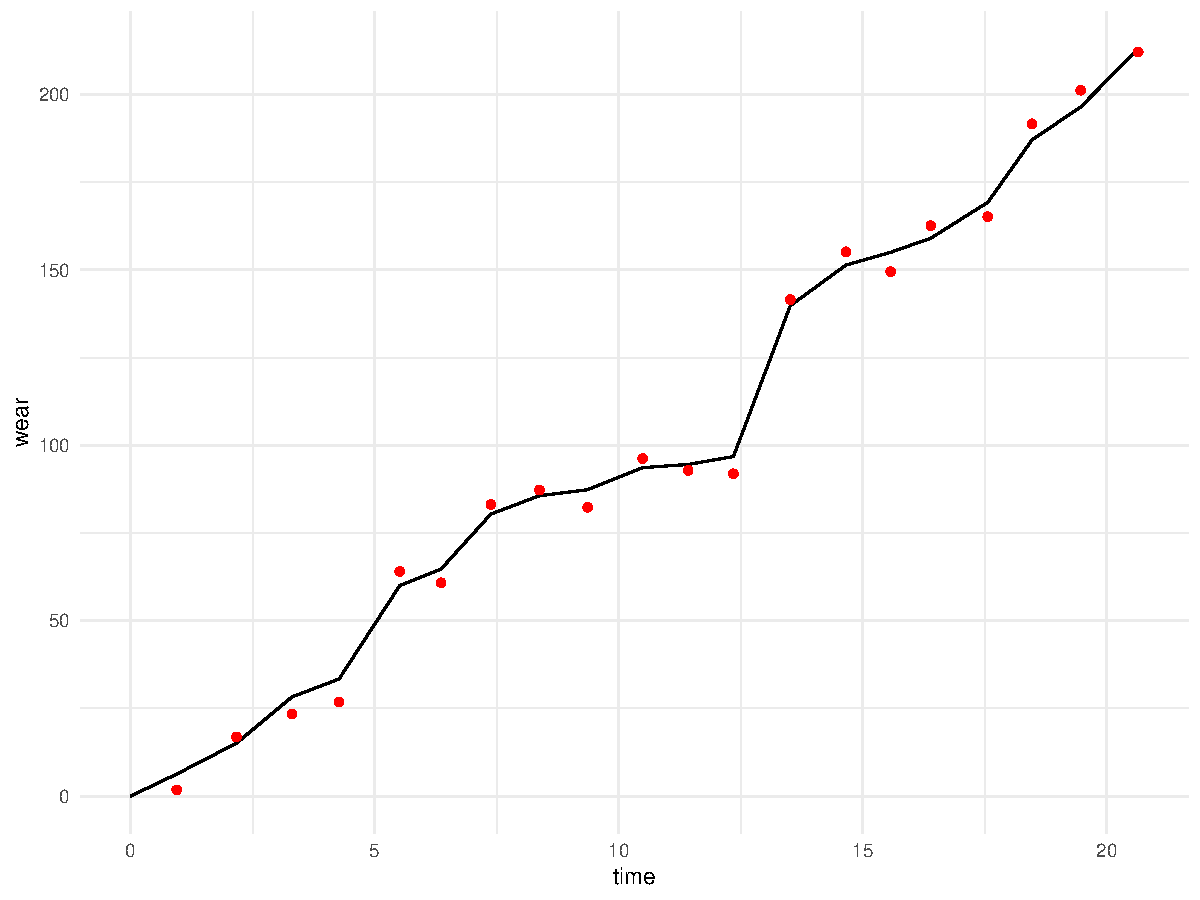
\includegraphics[width=0.95\textwidth]{./figures/ch-4/SimData.pdf}
  \caption{A simulated degradation trace (black) generated from a gamma process with parameters $\mu = 10$ and $\nu = 1.119$ and the simulated noisy observations (red) of the trace.}
  \label{fig:sim-data}
\end{figure}

\section{Constructing the prior} \label{sec:GP_priors}

The prior distribution in the parameter model summarises our beliefs about the parameters. There are two ways this information is encoded: the choice of distribution and the values of the hyperparameters. Before the advent of contemporary sampling algorithms, Bayesian analysis relied on conjugate prior distributions, or convenient prior distributions that facilitated the use of Gibbs samplers or conventional Metropolis-Hastings algorithms \citep{gilks_1996}. However, with the development of more efficient sampling algorithms such as Hamiltonian Monte Carlo \citep{betancourt_2017}, we are no longer limited by such requirements and can select priors that reflect our state of knowledge, facilitate efficient computation, and that can be justified and evaluated in a principled way. In this section, I compare some commonly used `default' priors for the GP from the reliability literature with a set of well-thought-out priors for the new parameters through prior predictive simulation: along the way, I provide justification for the new choice of priors for the alternative parameters $\mu$ and $\nu$.

In the degradation modelling literature, a gamma distribution is often used as the prior distribution for the rate parameter $\xi$ of the gamma process \citep{lawless2004} and also for the shape parameter \citep{rodriguez-picon2018}. It is well known that a gamma prior on the rate parameter is conditionally conjugate \citep{pradhan2011}, and its use leads to analytically tractable results, as \cite{lawless2004} show. Nevertheless, little work has been done to assess whether other prior distributions might be more appropriate. The gamma distribution has a heavy tail, and its use can lead to MCMC chains that converge very slowly or that are highly autocorrelated; moreover, it can lead to physically implausible realisations of the gamma process, as I demonstrate below. Using the new parameterisation of the GP in terms of $\mu$ and $\nu$, conditional conjugacy no longer exists, and so there is even less motivation for a gamma prior.

\begin{figure}
  \centering
  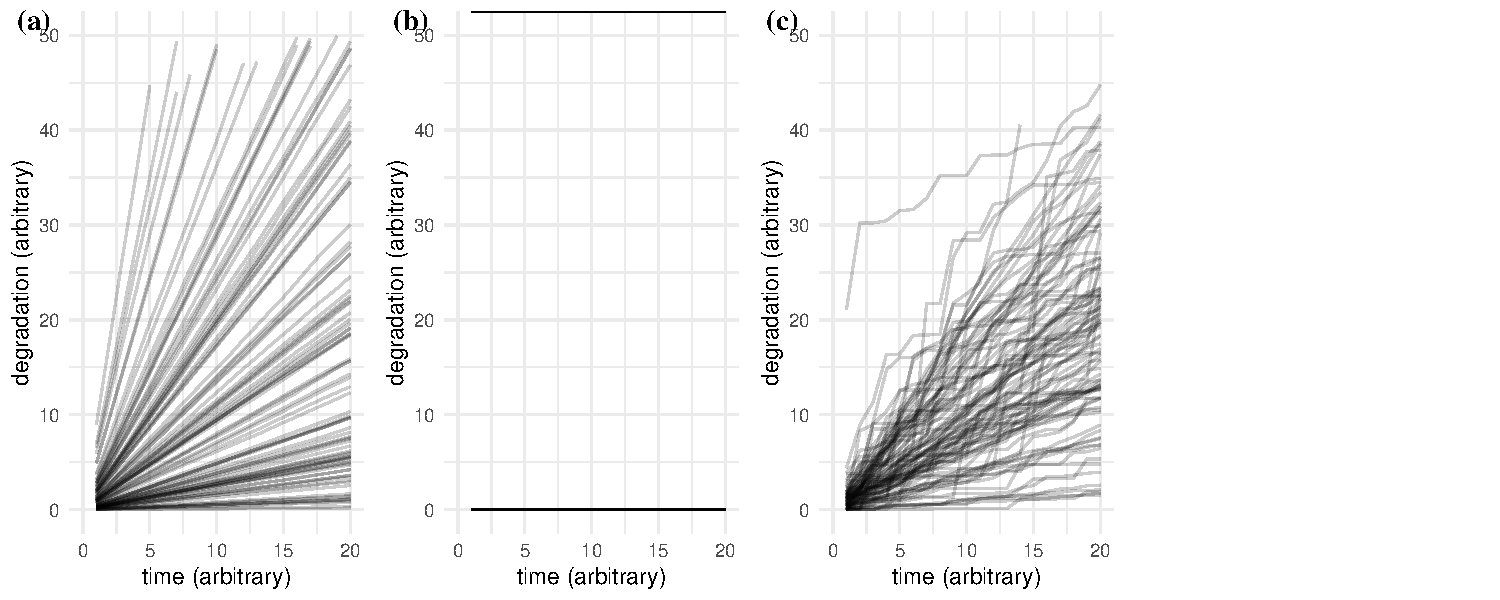
\includegraphics[width=1.2\textwidth]{./figures/ch-4/PPCs.pdf}
  \caption{One hundred realizations from prior predictive distributions of a noise-free gamma process with mean degradation rate of 1 unit per unit time and different prior distributions for parameters: (a) shape, rate $\sim \mbox{Ga}(1, 0.001)$, (b) shape, rate $\sim \mbox{Ga}(0.001, 0.001)$, and (c) parameterization mean/coefficient of variation---see text for details.}
  \label{fig:ppc}
\end{figure}

In Figure~\ref{fig:ppc}, I illustrate prior predictive checking of a noise-free gamma process using three sets of priors for its parameters: first, `conventional' priors, $\mbox{Ga}(1, 0.001)$ and $\mbox{Ga}(0.001, 0.001)$, that are widely used in the literature for both the shape and rate parameters of the usual parameterisation of a noise-free gamma process in eq.~\eqref{eq:GP_stationary}, and second, priors on $\mu$ and $\nu$ in the alternative parameterisation of eq.~\eqref{eq:GP_stationary_reparam} with carefully thought out weakly informative priors. All three sets of priors yield an average degradation rate of 1 unit per unit time. 

The distribution $\mbox{Ga}(\epsilon, \tilde{\epsilon})$, where $\epsilon, \tilde{\epsilon}\longrightarrow 0$, is often used as a noninformative prior distribution, especially in mixed linear models, where it is a conditionally conjugate prior for the precision \citep[p.~33]{hodges_2014}. In addition, as I pointed out above, the gamma distribution is conditionally conjugate for the rate parameter: if $\{ z_i \}$, $i = 1, 2, \ldots, n$, represents an independent sample from $\mbox{Ga}(\beta, \xi)$, then the conditional distribution of $\xi$ given $\beta$ and the data is $\mbox{Ga}(n\beta + \epsilon, \sum_{i=1}^n z_i + \tilde{\epsilon})$ when the prior distribution of $\xi$ is $\mbox{Ga}(\epsilon, \tilde{\epsilon})$. Hence, when $\epsilon$ and $\tilde{\epsilon}$ are both small, the prior adds very little information, but it is noninformative \textit{with respect to the rate parameter only}; furthermore, inferences about $\xi$ may be sensitive to the values of $\epsilon$ and $\tilde{\epsilon}$ in data sets where small values of $\xi$ may be possible \citep[p.~130]{gelman_workflow_2020}. When $\mbox{Ga}(\epsilon, \tilde{\epsilon})$ is used for \textit{both} parameters, we can no longer assume that the joint prior will be noninformative and, therefore must evaluate it to determine whether it is indeed diffuse. For further discussion on the consequences of using $\mbox{Ga}(\epsilon, \tilde{\epsilon})$ as a prior distribution and guidance on using more sensible alternatives, see \cite{hodges_2014} and \cite{gelman_workflow_2020}.

Figure~\ref{fig:ppc}~(a) and (b) show 100 draws from the prior predictive distribution of a noise-free gamma process when both the shape and rate parameters are assigned the prior distribution $\mbox{Ga}(1, 0.001)$ (Fig.~\ref{fig:ppc}~(a)) or $\mbox{Ga}(0.001, 0.001)$ (Fig.~\ref{fig:ppc}~(b)). In Fig.~\ref{fig:ppc}~(a), we can clearly see that the degradation traces resulting from a $\mbox{Ga}(1, 0.001)$ prior distribution are all nearly linear, without the jumps expected of gamma processes; furthermore, many of the rates of degradation are unrealistically high or unrealistically low. In Fig.~\ref{fig:ppc}~(b), where a $\mbox{Ga}(0.001, 0.001)$ prior is used, most of the prior predictive distribution has mass around implausibly low values of the average rate, and there is one unrealistically steep degradation trace. As I pointed out earlier, the gamma distribution is highly skewed and has heavy tails; consequently, depending on the values of the shape and rate, the prior can place mass on high, low, or both high and low values, resulting in simulated data that simply could not be observed in practice. By contrast, prior simulations generated according to the weekly-informative priors constructed with respect to the alternative parameters $\mu$ and $\nu$ in Fig.~\ref{fig:ppc}~(b) look much more plausible.

To specify independent prior distributions of the parameters $\mu$ and $\nu$ in the GP model in eq.~\eqref{eq:GP_stationary_reparam}, I adopt the approach introduced by \cite{Simpson_2017}: design priors that favour simpler models over more complex ones and that are consistent with domain knowledge. The mean $\mu$ controls the average degradation rate, similar to the action of the slope parameter in a linear degradation path model. There is no reason to believe that the variability about the mean degradation rate would be asymmetric, so a Gaussian distribution with a small standard deviation is both appropriate and convenient
\begin{equation*}
  \mu \sim \mbox{N}(1, 0.5).
\end{equation*}
The coefficient of variation $\nu$ is a measure of the volatility of the degradation process, and although we might expect some heterogeneity in the wear rate as degradation progresses, we do not expect the wear rate to be extremely volatile. Hence, a truncated Student's $t$-distribution with 3 degrees of freedom is used as a prior for $\nu$;
\begin{equation*}
  \nu \sim t_3^{+}(0, 1),
\end{equation*}
where the superscript $(+)$ denotes a truncated distribution whose lower bound is zero; furthermore, I use the location-scale form of a $t$ distribution with $n$ degrees of freedom, written as $t_n(\hbox{location}, \hbox{scale})$. This prior places a large mass near zero but still allows the posterior distribution to move away from zero. In addition, it has lighter tails than a gamma distribution and consequently does not give too much weight to extremely volatile degradation paths. Figure~\ref{fig:ppc}~(c) shows 100 draws from this parameter model for the reparameterised gamma process. The degradation traces have the appearance of paths expected from a gamma process; that is, there are discrete jumps between time points, in contrast to Fig.~\ref{fig:ppc}~(a), where all the traces are straight lines. Furthermore, more than half the degradation values at the end (eleventh time point) are between 6 and 16, as would be expected when the degradation varies around one. Finally, although there are some extreme realisations, there are only one or two that are completely implausible.

To fully specify the model, I also need to specify a prior for the standard deviation of the measurement error, $\sigma$. Following the recommendations of \citet[Chap.~17]{gelman_workflow_2020}, I use a vague $\hbox{Uniform}(0, A)$ prior for $\sigma$, where $A$ is chosen to be large relative to the expected scale of $\sigma$. I use such a vague prior for demonstration purposes. However, in practice, an analyst should have a reasonable grasp of the scale of the measurement error and should be able to specify a weakly informative prior; I do exactly this in Sec.~\ref{sec:comp-sols}. Because our initial prior on $\sigma$ is so vague, I do not include the measurement error in the prior predictive checking in Fig.~\ref{fig:ppc}.

Of course, had I used different values of the hyperparameters for the $\mbox{N}$ and $t_3^{+}$ priors, the appearance of the degradation traces in Fig.~\ref{fig:ppc}~(c) would have been different. For example, if I had specified a much more defuse prior for the mean wear rate, then no doubt unrealistically fast and slow wearing degradation traces would have been generated. It is only through the use of prior predictive checking to choose sensible values of the hyper-parameters in conjunction with suitable distributional forms of the priors that a well-justified prior is obtained.

\section{Fitting the noisy gamma process} \label{sec:NGP-fitting}

To improve our understanding of the noisy GP model, I fit the Bayesian hierarchical model outlined in Sec.~\ref{sec:NGP} with the priors defined in Sec.~\ref{sec:GP_priors} to the single simulated degradation trace in Fig.~\ref{fig:sim-data} as well as to a subset of the simulated degradation measurements. For clarity, the full model is
\begin{align*}
  y_i|z_i, \sigma & \sim \mbox{N}(z_i, \sigma)  && \mbox{data model} \\
  z_i & = \sum_{j=0}^i \Delta z_j && \mbox{process model} \\ 
  \Delta z_i|\mu, \nu & \sim \mbox{Ga} \left( \frac{\Delta t_i}{\nu^2}, \frac{1}{\mu \nu^2} \right) \\
  \mu & \sim \mbox{N}^{+}(10, 10) && \mbox{parameter model} \\
  \nu & \sim t_2^{+}(0, 1) \\
  \sigma & \sim \mbox{Unif}(0, 100).
\end{align*}
The single path example shows that the noisy GP is more difficult to fit than a noise-free GP model. When the sample size is small, the model struggles to separate the parameters describing the variance of the measurement error and the volatility of the underlying gamma process because there is not enough information in the data to do so. To demonstrate this problem with identifiability, I fit the BHM of two data sets: one `large' data set consisting of all 20 simulated noisy degradation measurements in Fig.~\ref{fig:sim-data}, and another `small' data set that is a subset of 10 points. I fit the BHM of the noisy GP outlined in Sections~\ref{sec:NGP} and \ref{sec:GP_priors} to these two data sets and evaluate how well the true parameter values and underlying degradation path is reclaimed in the two resulting posterior distributions. I also investigate the efficiency of the No-U-Turn sampler for the two cases.

\subsection{Data simulation}

I generate the degradation trace in Fig.~\ref{fig:sim-data}---which I coin the `large' dataset---by first sampling twenty time increments from a $\mbox{Unif}(0.8, 1.3)$ distribution. Next, twenty jumps in degradation are sampled from $\mbox{Ga}(\Delta t_i/\nu^2, 1/\mu\nu^2)$, using $\mu = 10$ and $\nu = 1.119$. I then calculate the cumulative sum of the jumps to obtain the underlying, noise-free degradation trace $z_i$, where $z_0 = 0$ at $t_0 = 0$. Finally, I add Gaussian noise with standard deviation $\sigma = 4$ to the underlying degradation path to get the noisy observations. The big dataset is described in Tab.~\ref{tab:big_df}. To create the second smaller data set, ten of the twenty noisy observations are randomly selected. The selected degradation observations that make up the small data set are highlighted in red in Fig.~\ref{fig:sim-data-small} and displayed in Tab.~\ref{tab:small_df}.

\begin{figure}
  \centering
  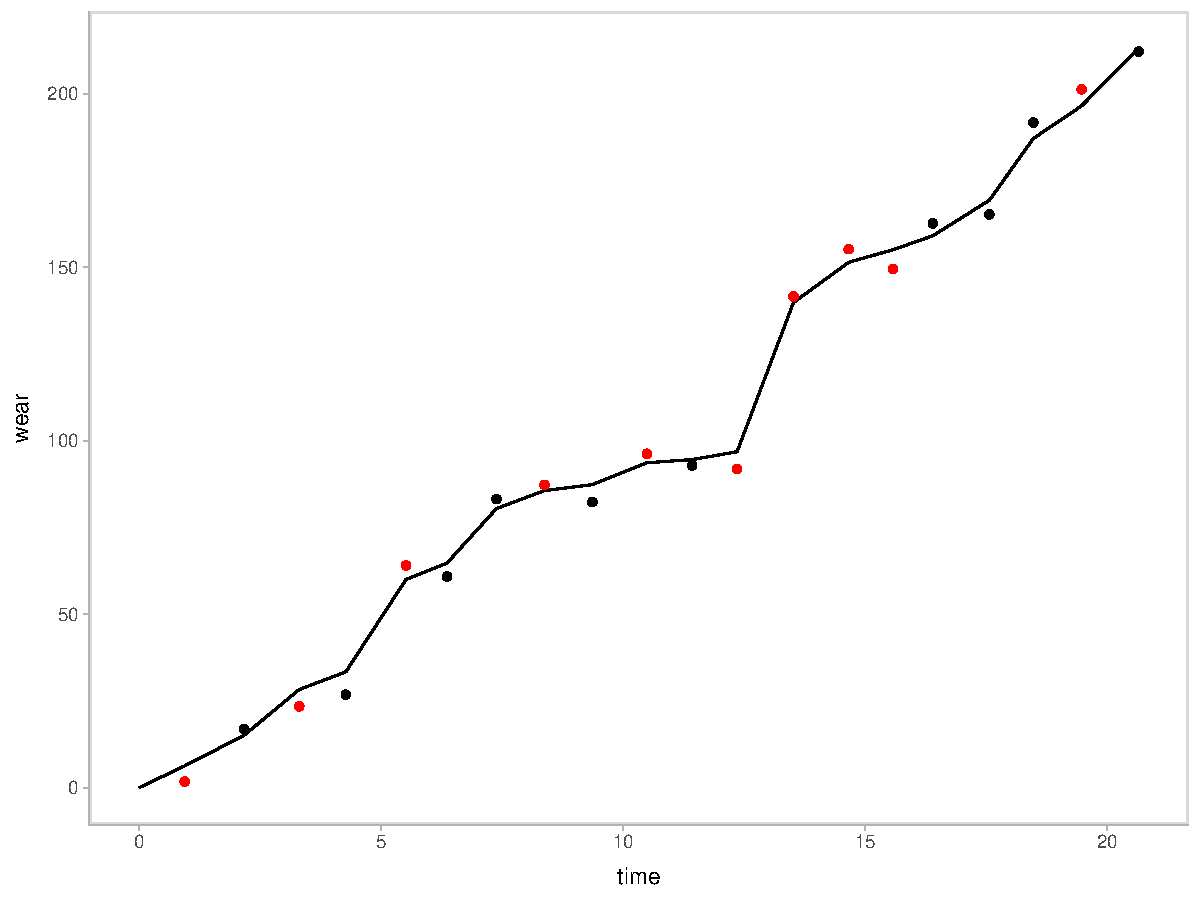
\includegraphics[width=0.95\textwidth]{./figures/ch-4/SimData_big_small.pdf}
  \caption{The simulated degradation trace with the subset of observations selected for the small dataset highlighted in Red.}
  \label{fig:sim-data-small}
\end{figure}

\begin{table}
\centering
\caption{\label{tab:big_df}The twenty simulated noisy degradation observation that make up the `large' data set.}
\centering
\begin{tabular}[t]{rrrr}
\toprule
$t$ & $\Delta z$ & $z$ & $y$\\
\midrule
\cellcolor{gray!10}{0.00} & \cellcolor{gray!10}{NA} & \cellcolor{gray!10}{0.00} & \cellcolor{gray!10}{NA}\\
0.95 & 6.29 & 6.29 & 1.77\\
\cellcolor{gray!10}{2.17} & \cellcolor{gray!10}{8.81} & \cellcolor{gray!10}{15.10} & \cellcolor{gray!10}{16.87}\\
3.31 & 13.20 & 28.30 & 23.42\\
\cellcolor{gray!10}{4.27} & \cellcolor{gray!10}{5.09} & \cellcolor{gray!10}{33.39} & \cellcolor{gray!10}{26.80}\\
\addlinespace
5.52 & 26.63 & 60.02 & 64.04\\
\cellcolor{gray!10}{6.36} & \cellcolor{gray!10}{4.73} & \cellcolor{gray!10}{64.75} & \cellcolor{gray!10}{60.84}\\
7.38 & 15.66 & 80.41 & 83.15\\
\cellcolor{gray!10}{8.38} & \cellcolor{gray!10}{5.21} & \cellcolor{gray!10}{85.62} & \cellcolor{gray!10}{87.24}\\
9.36 & 1.71 & 87.33 & 82.31\\
\addlinespace
\cellcolor{gray!10}{10.49} & \cellcolor{gray!10}{6.30} & \cellcolor{gray!10}{93.63} & \cellcolor{gray!10}{96.23}\\
11.43 & 0.92 & 94.54 & 92.85\\
\cellcolor{gray!10}{12.35} & \cellcolor{gray!10}{2.25} & \cellcolor{gray!10}{96.79} & \cellcolor{gray!10}{91.88}\\
13.52 & 43.01 & 139.80 & 141.53\\
\cellcolor{gray!10}{14.66} & \cellcolor{gray!10}{11.57} & \cellcolor{gray!10}{151.37} & \cellcolor{gray!10}{155.16}\\
\addlinespace
15.57 & 3.63 & 155.00 & 149.48\\
\cellcolor{gray!10}{16.40} & \cellcolor{gray!10}{4.02} & \cellcolor{gray!10}{159.02} & \cellcolor{gray!10}{162.60}\\
17.56 & 10.23 & 169.26 & 165.16\\
\cellcolor{gray!10}{18.47} & \cellcolor{gray!10}{17.79} & \cellcolor{gray!10}{187.05} & \cellcolor{gray!10}{191.65}\\
19.47 & 9.40 & 196.44 & 201.20\\
\addlinespace
\cellcolor{gray!10}{20.65} & \cellcolor{gray!10}{16.57} & \cellcolor{gray!10}{213.01} & \cellcolor{gray!10}{212.11}\\
\bottomrule
\end{tabular}
\end{table}


\begin{table}
\centering
\caption{\label{tab:small_df}The subset of ten simulated noisy degradation observation from the `big' data set which make up the `small' data set.}
\centering
\begin{tabular}[t]{rrrr}
\toprule
$t$ & $\Delta z$ & $z$ & $y$\\
\midrule
\cellcolor{gray!10}{0.00} & \cellcolor{gray!10}{NA} & \cellcolor{gray!10}{0.00} & \cellcolor{gray!10}{NA}\\
0.95 & 6.29 & 6.29 & 1.77\\
\cellcolor{gray!10}{3.31} & \cellcolor{gray!10}{13.20} & \cellcolor{gray!10}{28.30} & \cellcolor{gray!10}{23.42}\\
5.52 & 26.63 & 60.02 & 64.04\\
\cellcolor{gray!10}{8.38} & \cellcolor{gray!10}{5.21} & \cellcolor{gray!10}{85.62} & \cellcolor{gray!10}{87.24}\\
\addlinespace
10.49 & 6.30 & 93.63 & 96.23\\
\cellcolor{gray!10}{12.35} & \cellcolor{gray!10}{2.25} & \cellcolor{gray!10}{96.79} & \cellcolor{gray!10}{91.88}\\
13.52 & 43.01 & 139.80 & 141.53\\
\cellcolor{gray!10}{14.66} & \cellcolor{gray!10}{11.57} & \cellcolor{gray!10}{151.37} & \cellcolor{gray!10}{155.16}\\
15.57 & 3.63 & 155.00 & 149.48\\
\addlinespace
\cellcolor{gray!10}{19.47} & \cellcolor{gray!10}{9.40} & \cellcolor{gray!10}{196.44} & \cellcolor{gray!10}{201.20}\\
\bottomrule
\end{tabular}
\end{table}


\subsection{Computation}

To sample from the posteriors of the noisy GP model conditioned on the two different datasets I use the No-U-Turn sampler. I generated $88,000$ samples from each posterior distribution using four chains of $25,000$ iterations each, with a burn-in of $3,000$ and no thinning. To ensure a detailed exploration of the posterior, I also change the sampling parameters \textit{adapt delta} and \textit{maximum tree depth} to $0.99$ and $13$ respectively. Raising \textit{adapt delta} results in a more aggressive (smaller) choice of the step size for the leapfrog algorithm that approximates the Hamiltonian trajectories, and raising the \textit{maximum tree depth} allows each leapfrog algorithm to run for longer. Increasing these two sampling parameters results in a slower sampler but ensures a more detailed exploration of the posterior when there are areas of tight curvature. All of the code to define the model in Stan, simulate the data in R, and sample from the posterior using RStan is available on the GitHub repository for the Thesis.

During sampling---despite increasing \textit{adapt delta} and \textit{maximum tree depth}---eighty divergent transitions occur while fitting the model to the small data set, whereas only four occur when sampling from the posterior conditioned on the larger data set. The divergencies signify incomplete exploration of the target distribution, which I explore in the next section. In addition to evaluating sampling through divergent transitions, energy diagnostics quantify the heaviness of the tails of the posterior distribution and thus can identify inefficient sampling \citep{bayesplot}. The chain energy plots in Fig.~\ref{fig:nuts-energies} compare the marginal energy distribution, $\pi_E$, with the first differenced distribution, $\pi_{\Delta E}$, for each chain. These plots are similar to those in \citet{betancourt_2017} that compare the energy transition distribution (equivalent to $\pi_{\Delta E}$) with the marginal energy distribution (equivalent to $\pi_E$). Ideally, these two overlaid distributions should look the same. However, if the distribution of $\pi_{\Delta E}$ is much narrower than that of $\pi_E$, like it is in Fig~\ref{fig:nuts-energies}~(b), then this indicates slow exploration of the target distribution. The energy diagnostics from fitting the model to the small data set in Fig.~\ref{fig:nuts-energies}~(b) show that exploration of the posterior is very inefficient, whereas when fitting the model to the big dataset, Fig.~\ref{fig:nuts-energies}~(a), sampling is much more efficient---although it is not perfect. The number of flagged divergent transitions and the energy plots are warning signs of an issue with the model, they do not diagnose the issue. Section~\ref{sec:noisy-GP-results} looks more closely at the posterior draws and divergent transitions to properly identify the issues with the model.

\begin{figure}
  \centering
  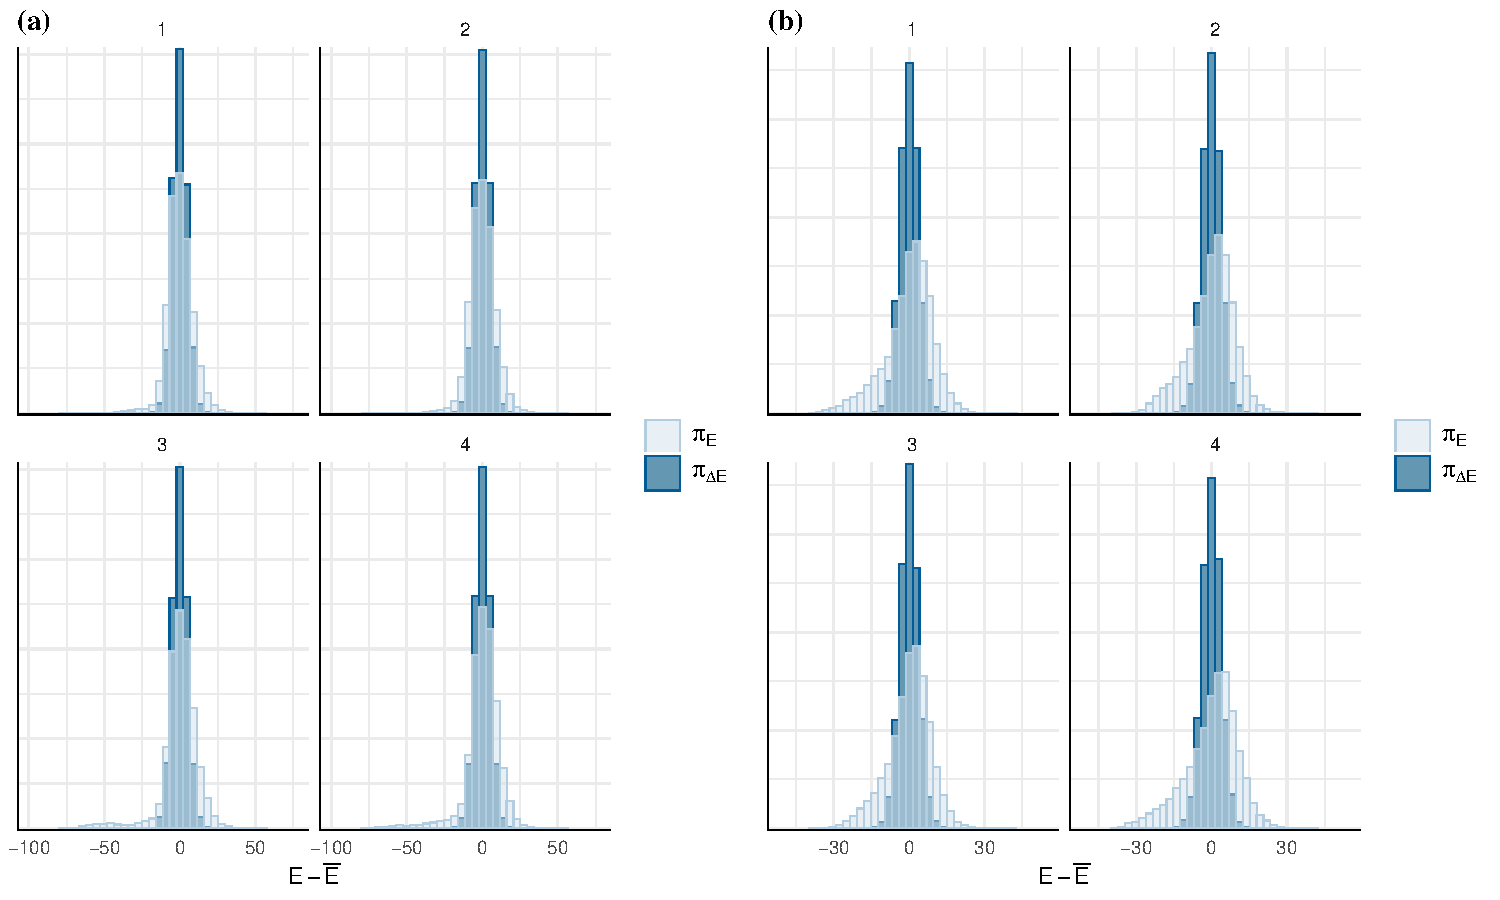
\includegraphics[width=0.95\textwidth]{./figures/ch-4/nuts_energy.pdf}
  \caption{The chain energy diagnostics for each chain when sampling from the posterior of the big data set (left) and small data set. Each plot compares the marginal energy distribution, $\pi_E$, with the first differenced distribution, $\pi_{\Delta E}$.}
  \label{fig:nuts-energies}
\end{figure}

\subsection{Results and diagnostics} \label{sec:noisy-GP-results}

My objective here is to investigate how the size of the dataset affects inference from the BHM for a noisy GP. To do so, I assess how well the parameters and underlying degradation trace are reclaimed in the two posterior distributions. Visualising the two posteriors shows that when the model is fitted to all twenty degradation observations, it is able to recover the parameter values and underlying degradation path; when only a subset of ten noisy observations is used, the model fails to do so because it is unable to disentangle the measurement error from the volatility of the underlying gamma process. I come to this conclusion by exploring the degenerate behaviours in the posterior that are flagged by divergent trajectories that occurred during sampling. 

\paragraph*{Marginal densities}
Figure~\ref{fig:marginal-post} shows the marginal distributions of the parameters $\mu$, $\nu$, and $\sigma$ conditioned on the small and big data sets as well as the true values of the parameters. For each marginal density, the median and 66\% and 95\% credible intervals are shown. It is clear that when the model is fit to the small data set, it fails to reclaim the true parameter values, but when fitted to the bigger dataset, it successfully reclaims the true values. The marginal posterior densities of the parameters conditioned on all twenty degradation observations are centred around the true values of the parameters, whereas the marginal posteriors of $\sigma$ and $\nu$ conditioned on the subset of ten observations are centred around fifteen and zero, respectively. Furthermore, the marginal posterior of $\sigma$ conditioned on the smaller subset of the data appears to have some multimodality. To understand the implication of these parameter estimates as well as the effect of how they covary with one another in the posterior I look at their joint effect on the outcome variables, which in this case is the predictive distribution of the filtered degradation path.

\begin{figure}
  \centering
  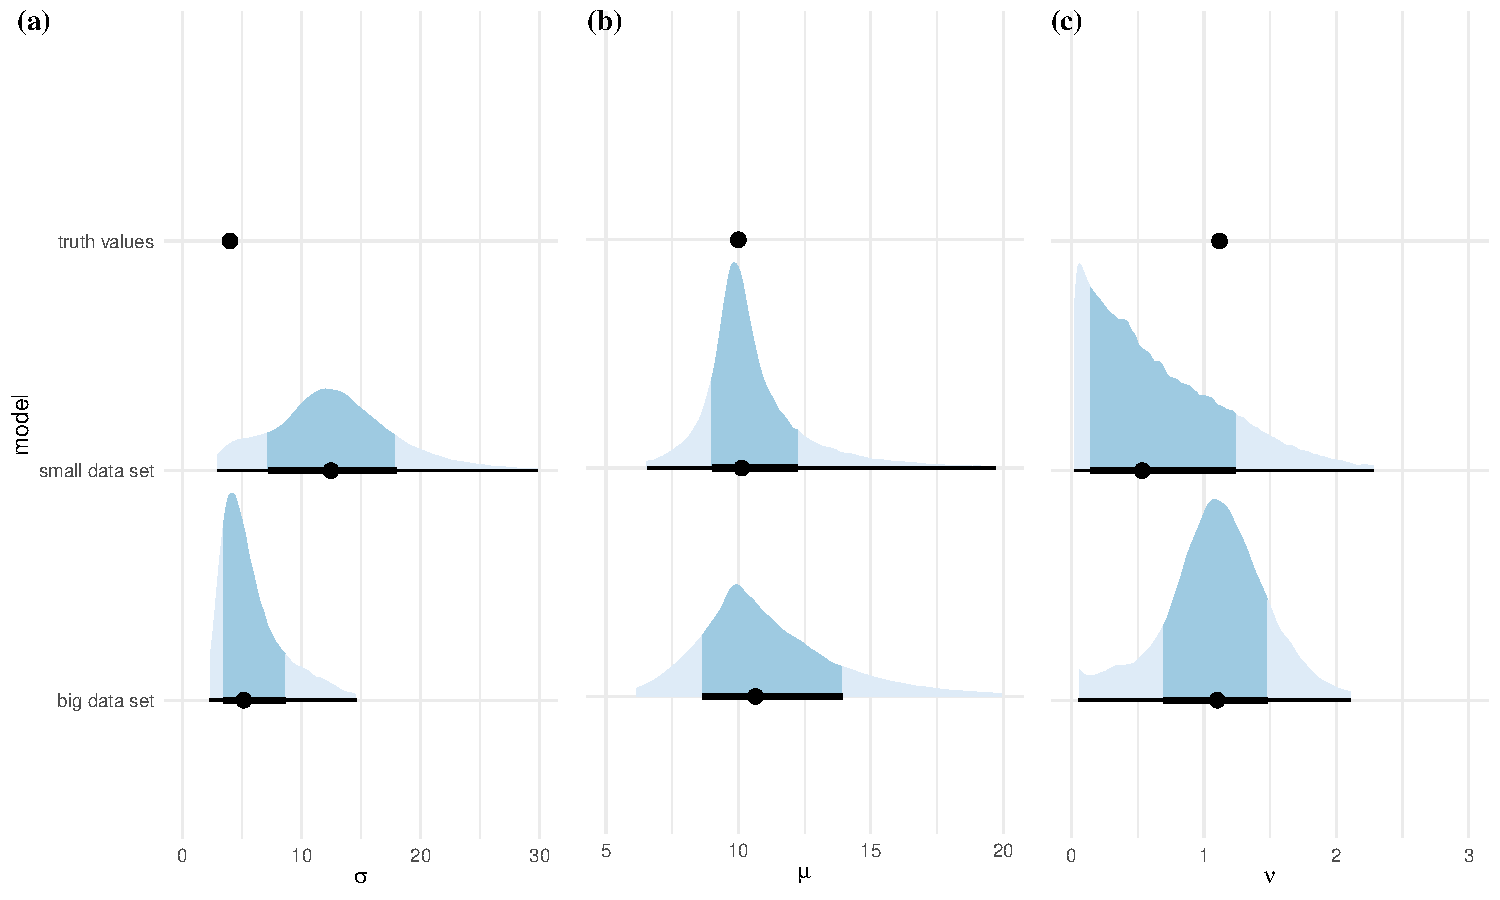
\includegraphics[width=0.95\textwidth]{./figures/ch-4/marginal-posterior_a.pdf}
  \caption{The marginal posterior distributions of the parameters $\sigma$, $\mu$, and $\nu$ when the BHM for the noisy gamma process is fitted to the `large' and `small' simulated data in Fig.~\ref{fig:sim-data}. The points and intervals shown in each distribution represent, respectively, the median and $95\%$ and $66\%$ credible intervals. The values used to simulate the data are shown in the top row.}
  \label{fig:marginal-post}
\end{figure}

\paragraph*{Posterior predictive density}
Figure~\ref{fig:ppd-z} shows the posterior predictive distribution of the underlying degradation trace, the $z_i$, for the two posteriors with the true degradation trace and noisy observations overlaid. The thick grey line in each plot is the median of the posterior predictive distribution; additional quantiles are shown in different shades of blue. Clearly, in Fig.~\ref{fig:ppd-z}~(a), the model has been able to reclaim the underlying degradation from the noisy degradation observations when fit to all twenty observations: the median path follows the actual path almost exactly, with uncertainty bands that are narrow enough to be useful. However, as was the case with parameter values, the median path derived from the posterior distribution conditioned on the subset of the data has not recovered the true path (Fig.~\ref{fig:ppd-z}~(b)). In Fig.~\ref{fig:ppd-z}~(b), the median path is a nearly straight line through the data points. In addition, the uncertainty intervals are much wider.

\begin{figure}
  \centering
  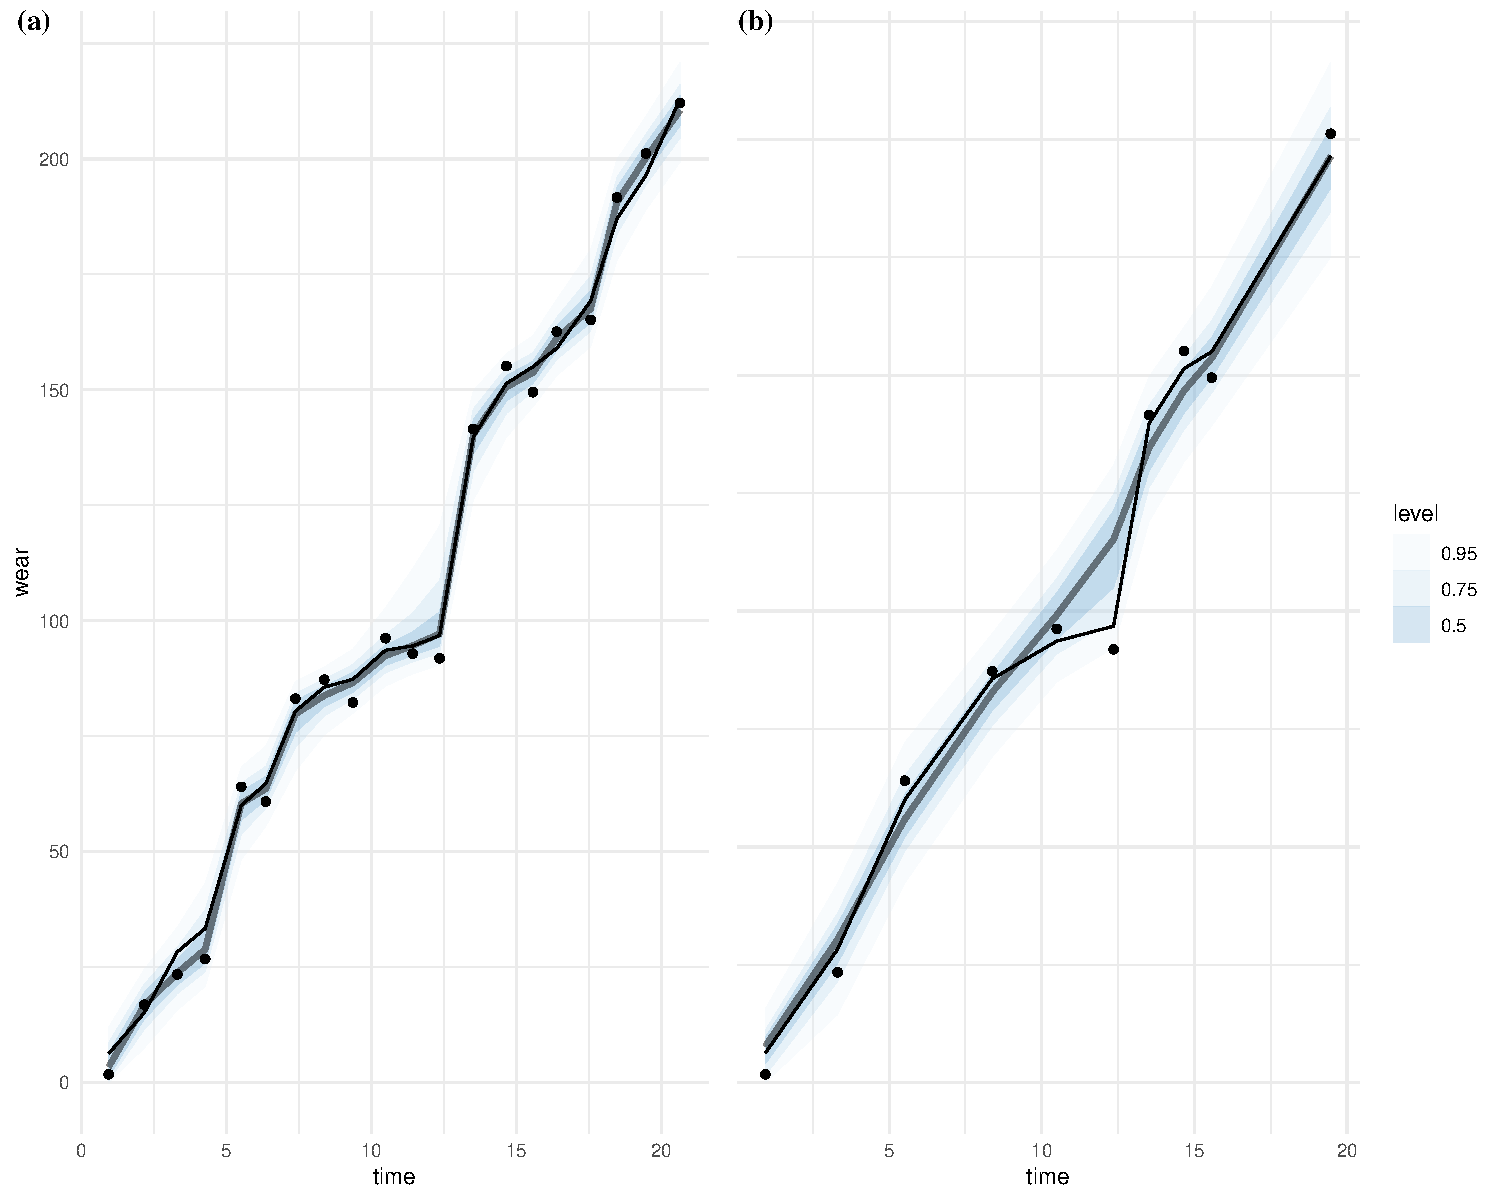
\includegraphics[width=0.95\textwidth]{./figures/ch-4/ppd_z_a.pdf}
  \caption{The posterior predictive distribution of the filtered degradation path compared to the true degradation path when (a) the model is fitted using the big and (b) small data set. If the distribution of $\pi_\text{E}$ is much wider that that of $\pi_{\Delta\text{E}}$, then sampling is inefficient.}
  \label{fig:ppd-z}
\end{figure}

\paragraph*{Pairs plots}
Clearly, some issues are occurring in the posterior distribution of the model conditioned on the smaller subset of the data. These issues were pre-eluded to by the divergent trajectories that occurred during sampling (Sec.~\ref{fig:pairs}). In the case of fitting the model to simulated data, where we can be sure that the model is properly specified and implemented, poorly behaved sampling is often a sign of a deeper issue with the model. As discussed in Sec.~\ref{sec:Bayesian-methods}, the divergent transitions can point to the problematic areas in the posterior. Figure~\ref{fig:pairs} shows a pairs plot of the parameters $\mu$, $\nu$, and $\sigma$ and the first degradation jump, $\Delta z_1$. The divergent trajectories are shown in red. In the bivariate scatter plots, there are strong funnel shapes between $\mu$ and $log(\nu)$ and between $log(\nu)$ and the first degradation jump. The divergent trajectories are concentrated at the entrance to these funnels, suggesting that they are the cause of the sampling issues. The funnel shapes occur because as $\nu$ shrinks towards zero $\mu$ and $\Delta z_1$ approach very particular values; $\mu = 10$ and $\Delta z_1 = 10 \times \Delta t_1$.

\begin{figure}
  \centering
  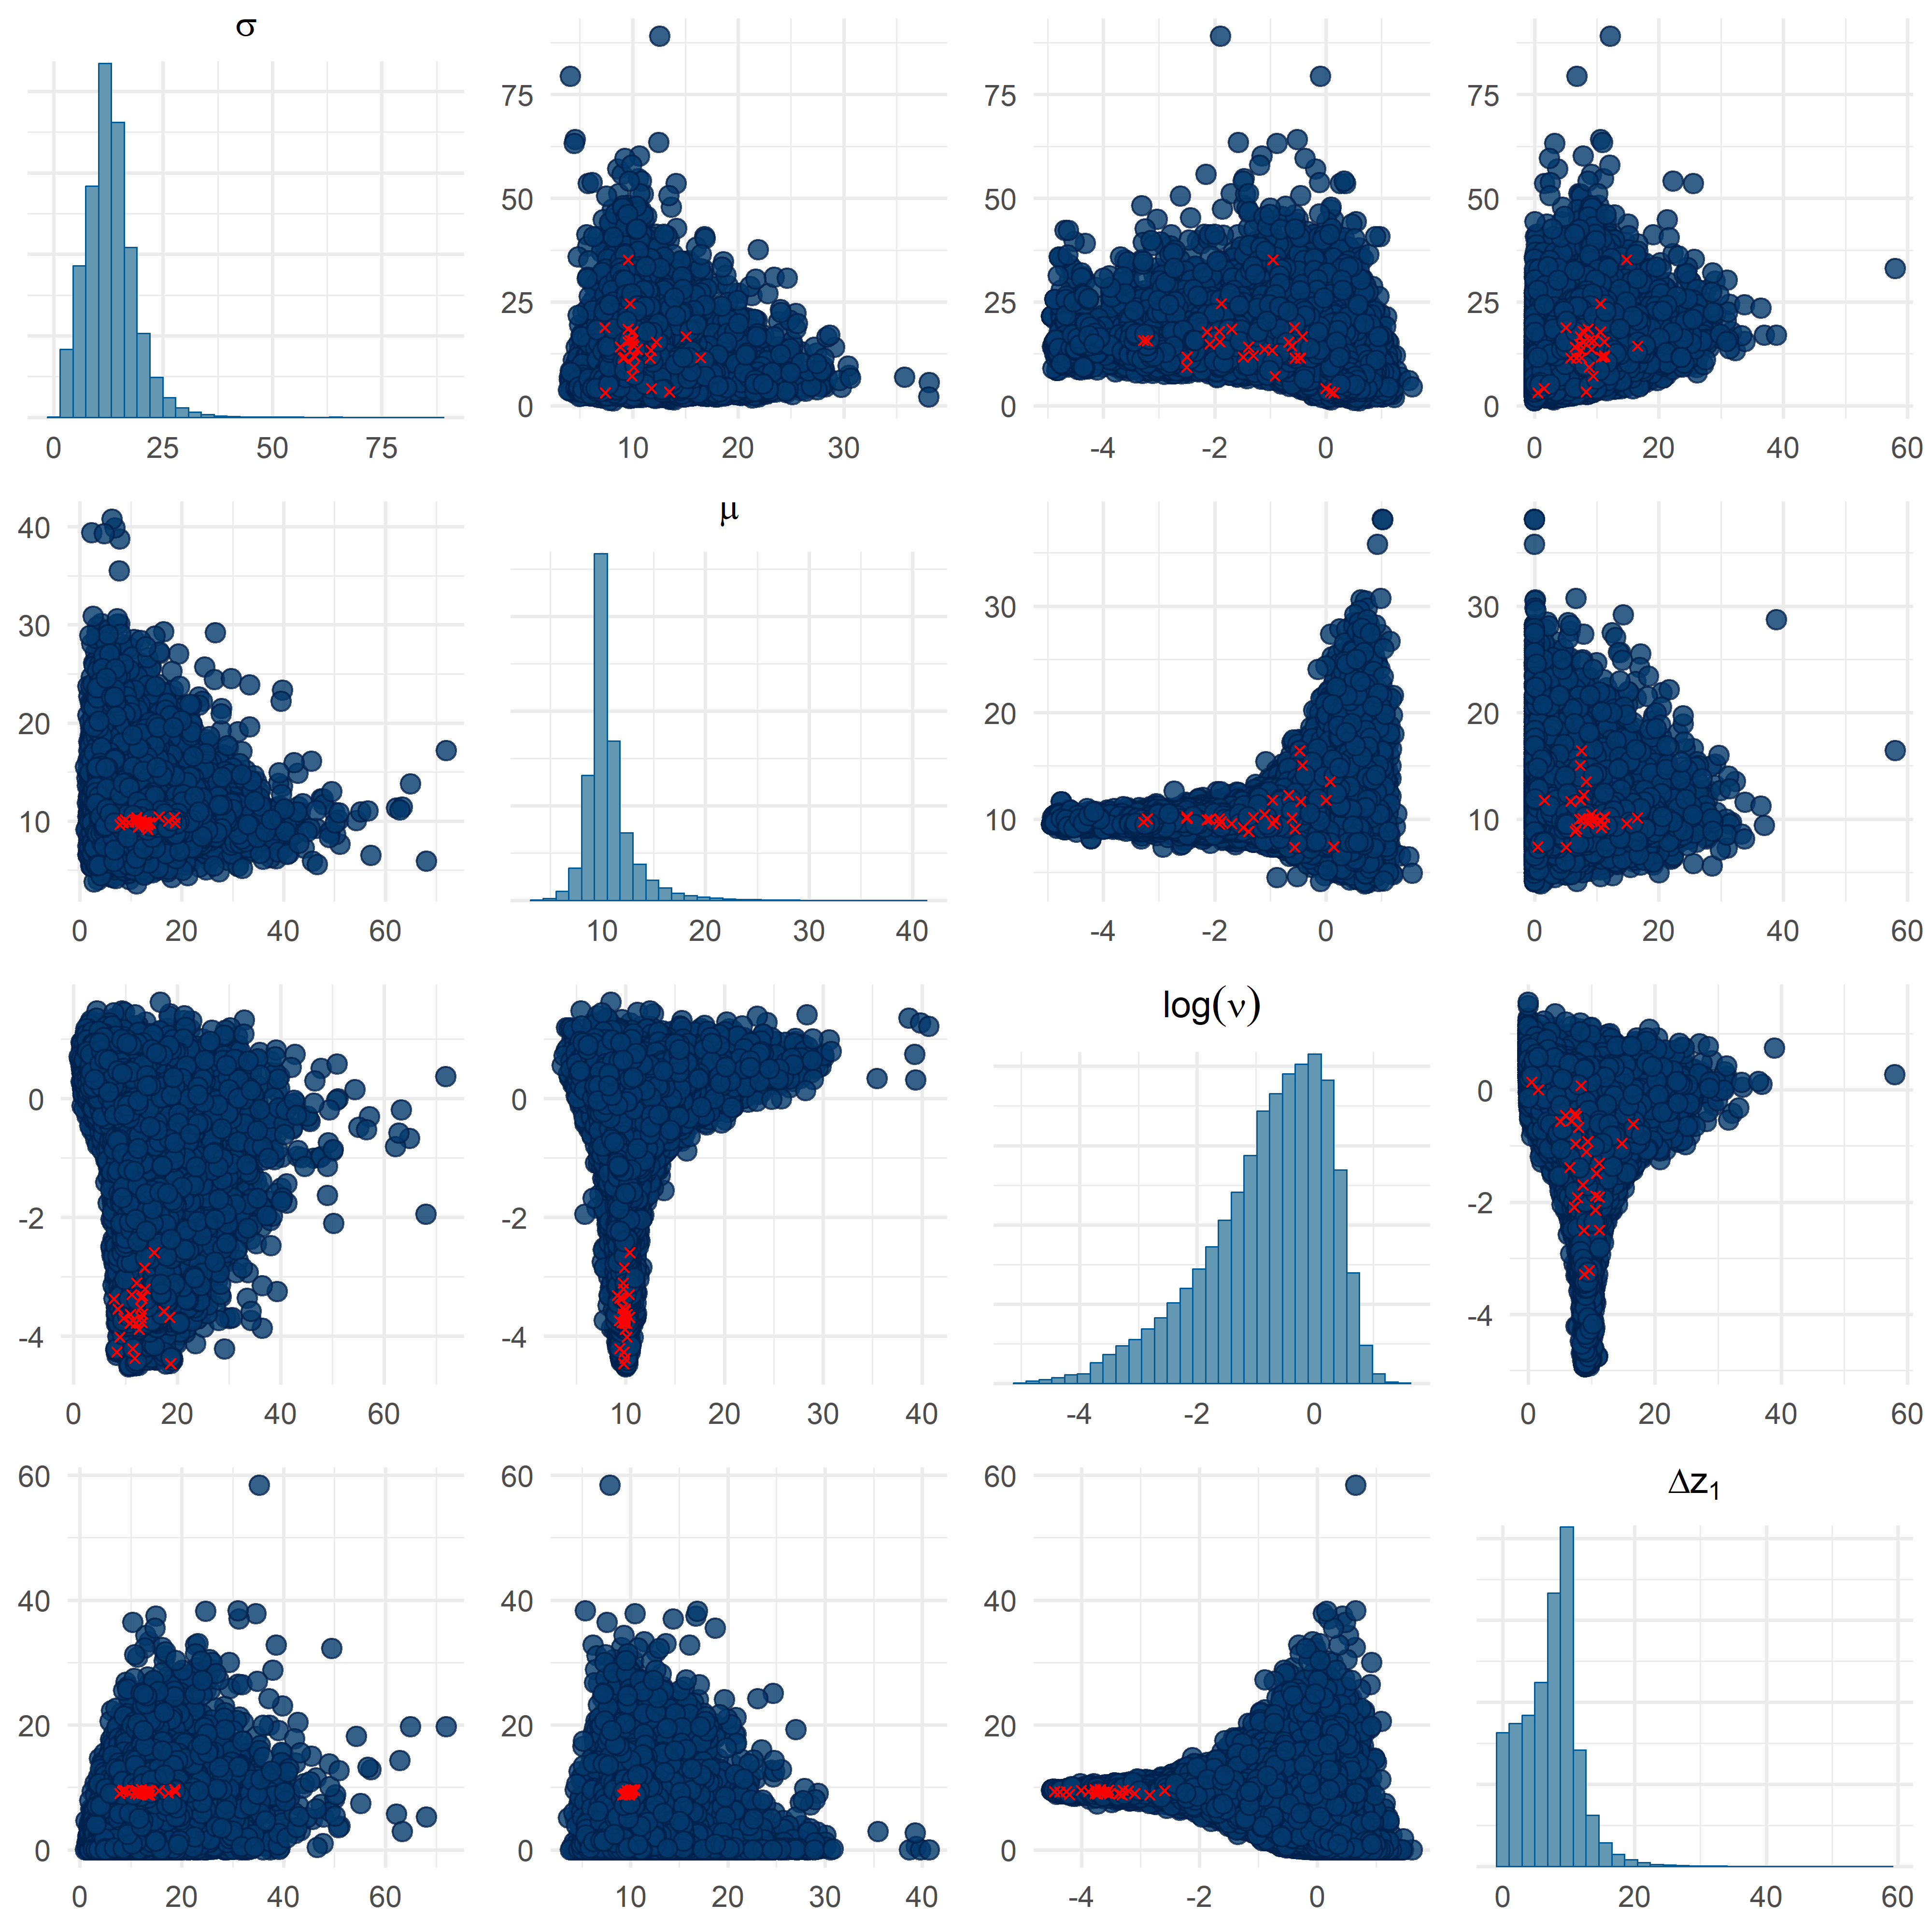
\includegraphics[width=0.95\textwidth]{./figures/ch-4/Small-data-pairs.png}
  \caption{Pairs plot showing the MCMC draws from the posterior distribution of the parameters $\sigma$, $\mu$, $\log\nu$, and the filtered value $\Delta z_1$ when the BHM of the noisy gamma process is fitted to the small dataset. The red points indicate divergences, which congregate at the end of the funnel in the pairwise plots of $\log\nu$/$\Delta z_1$ and $\log\nu$/$\mu$.}
  \label{fig:pairs}
\end{figure}

\paragraph*{Parallel coordinate plot}
The divergent trajectories can help to further explore how the degenerate behaviour manifests in the multidimensional posterior. Figure~\ref{fig:par-coord-single} shows a parallel coordinate plot of the posterior draws for all of the parameters in the model. The divergent trajectories are highlighted in red. The divergencies draw a clear structure through parameter space. They all pass through the values $\mu = 10$, $\nu = 0$, and $\Delta z_i = 10 \times \Delta t_i$ and an inflated value of $\sigma$ that is much larger than the true value $\sigma = 4$. This structure equates to a linear degradation trace with large measurement uncertainty. To emphasise this point, in Fig.~\ref{fig:z-ppd-divergent}, I plot the posterior predictive distribution of the underlying degradation path from the small data set and overlay the divergent paths. From this, it is clear that the areas of tight curvature in the posterior occur around the models where the degradation trace is effectively linear.

\begin{figure}
  \centering
  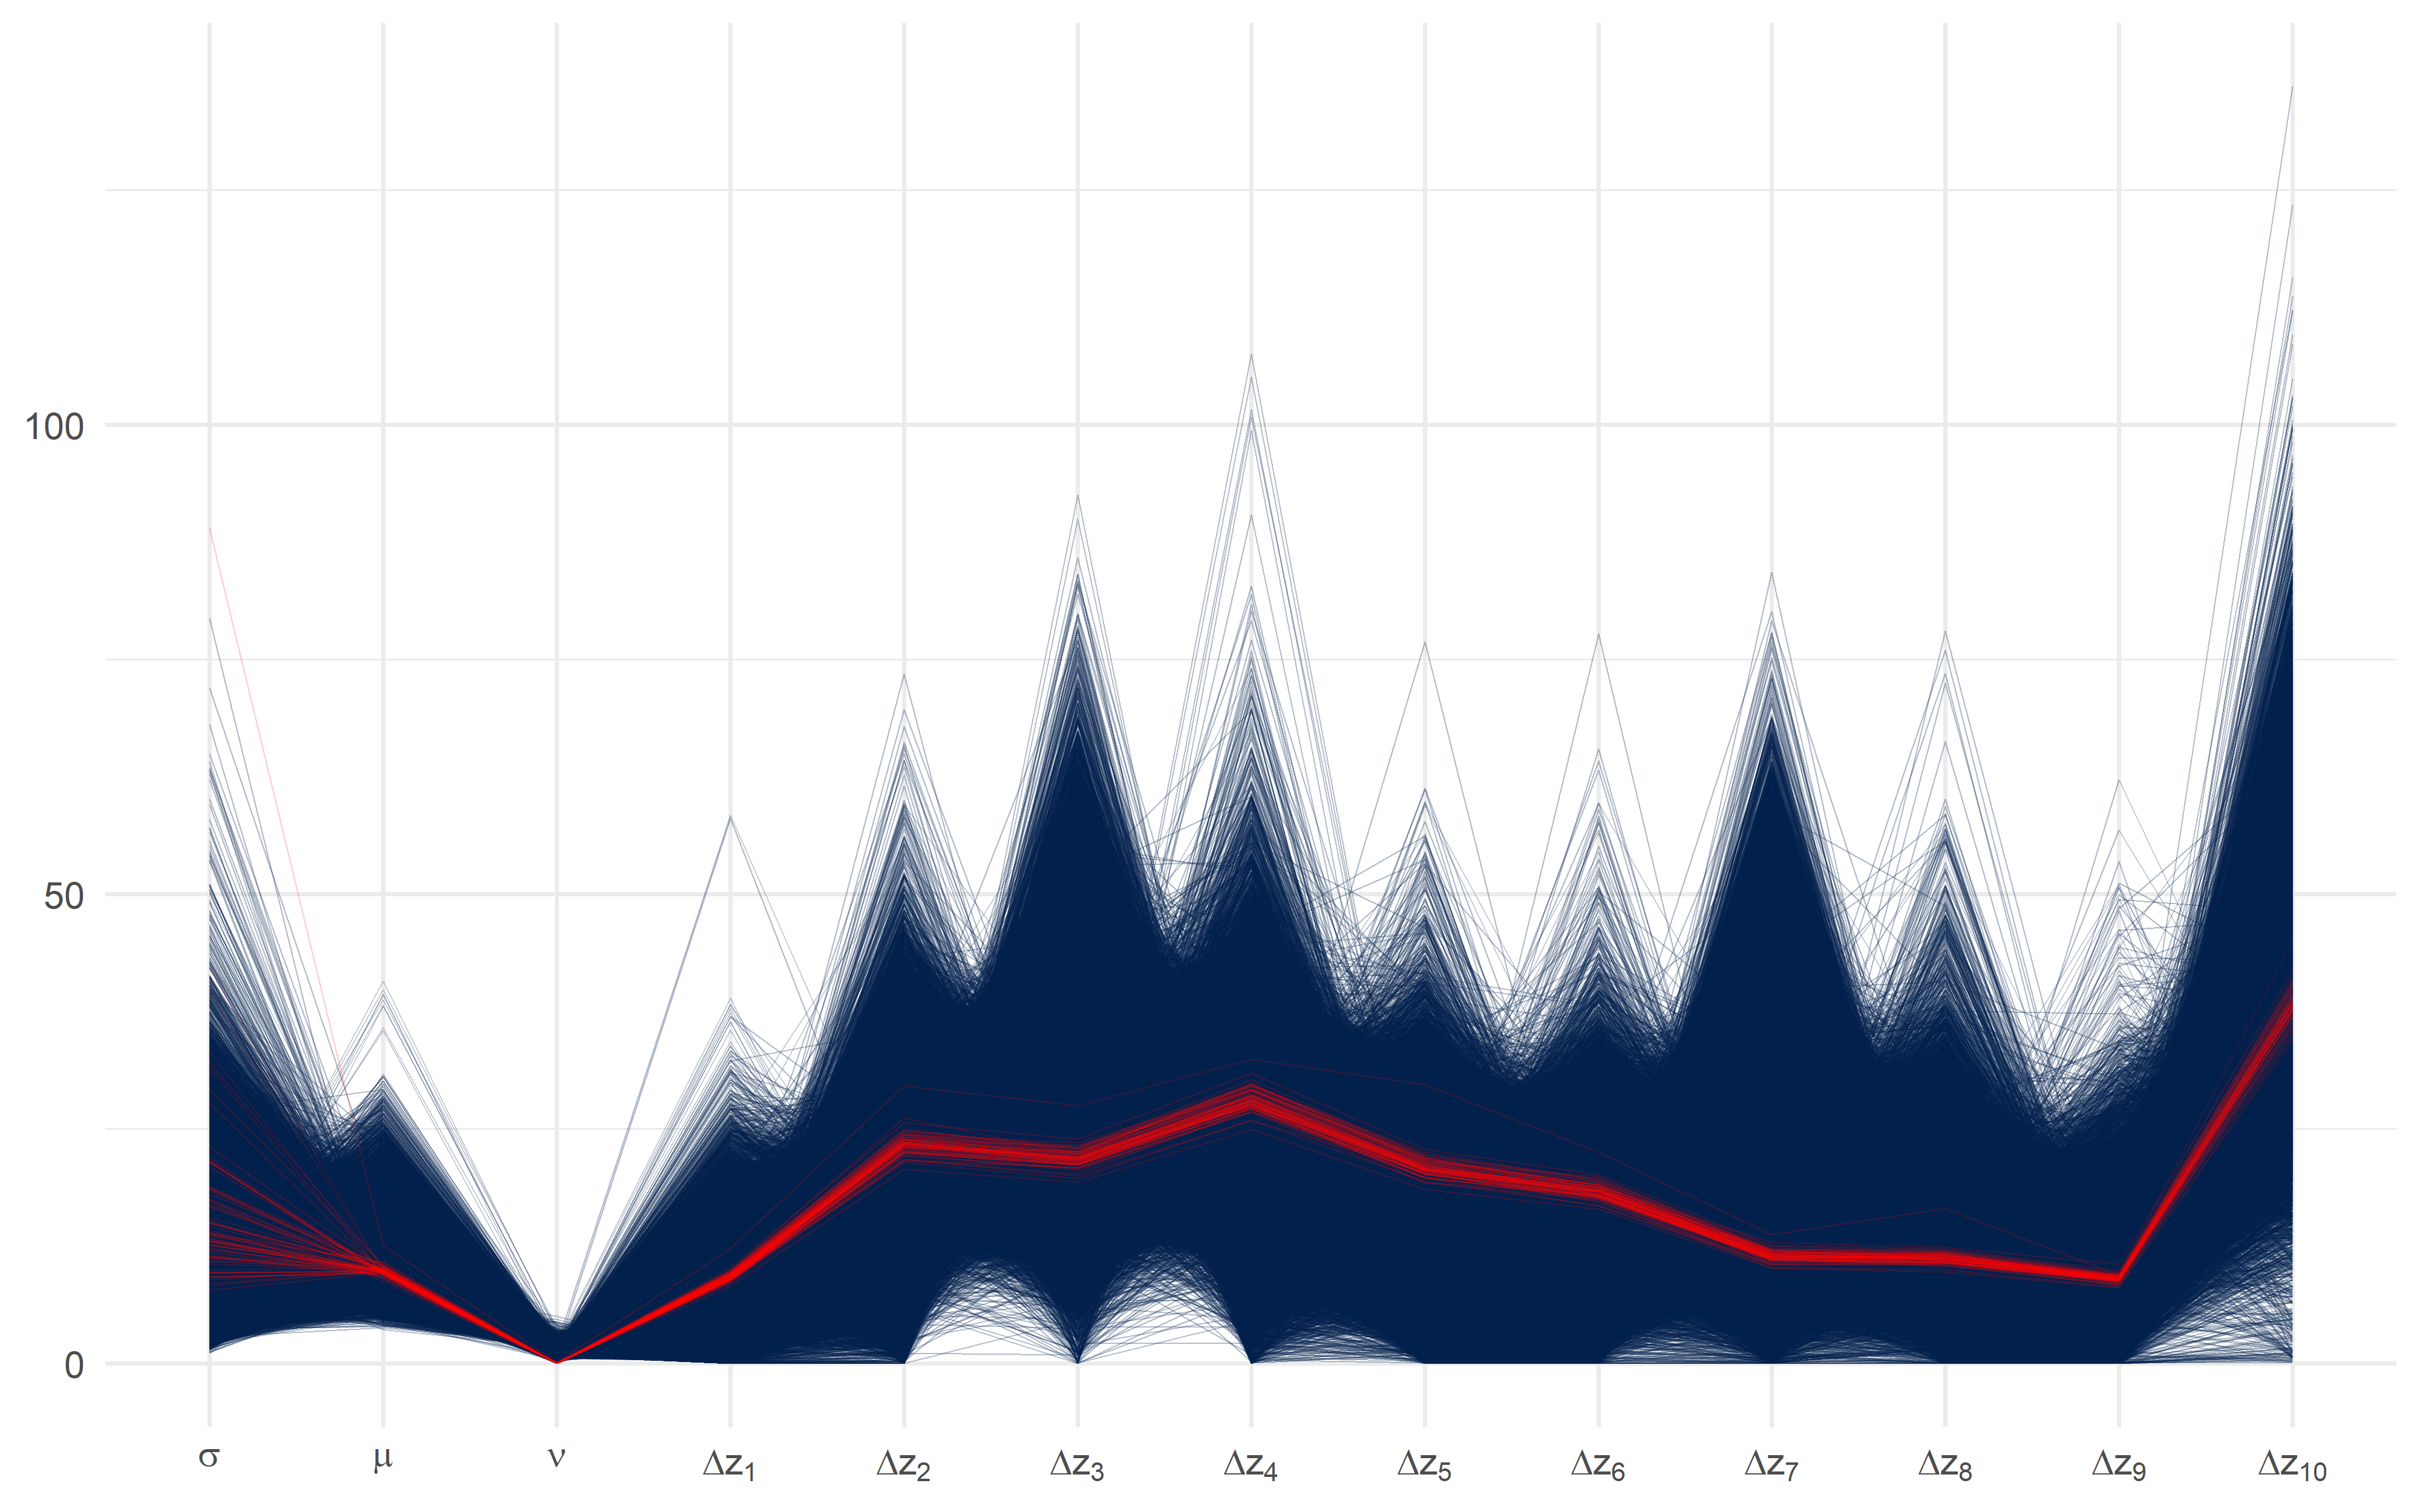
\includegraphics[width=0.8\columnwidth]{./figures/ch-4/parcoord.png}
  \caption{The parallel coordinate plot of the draws from the posterior conditioned on the small dataset with the divergent traces plotted in red.}
  \label{fig:par-coord-single}
\end{figure}

\begin{figure}
  \centering
  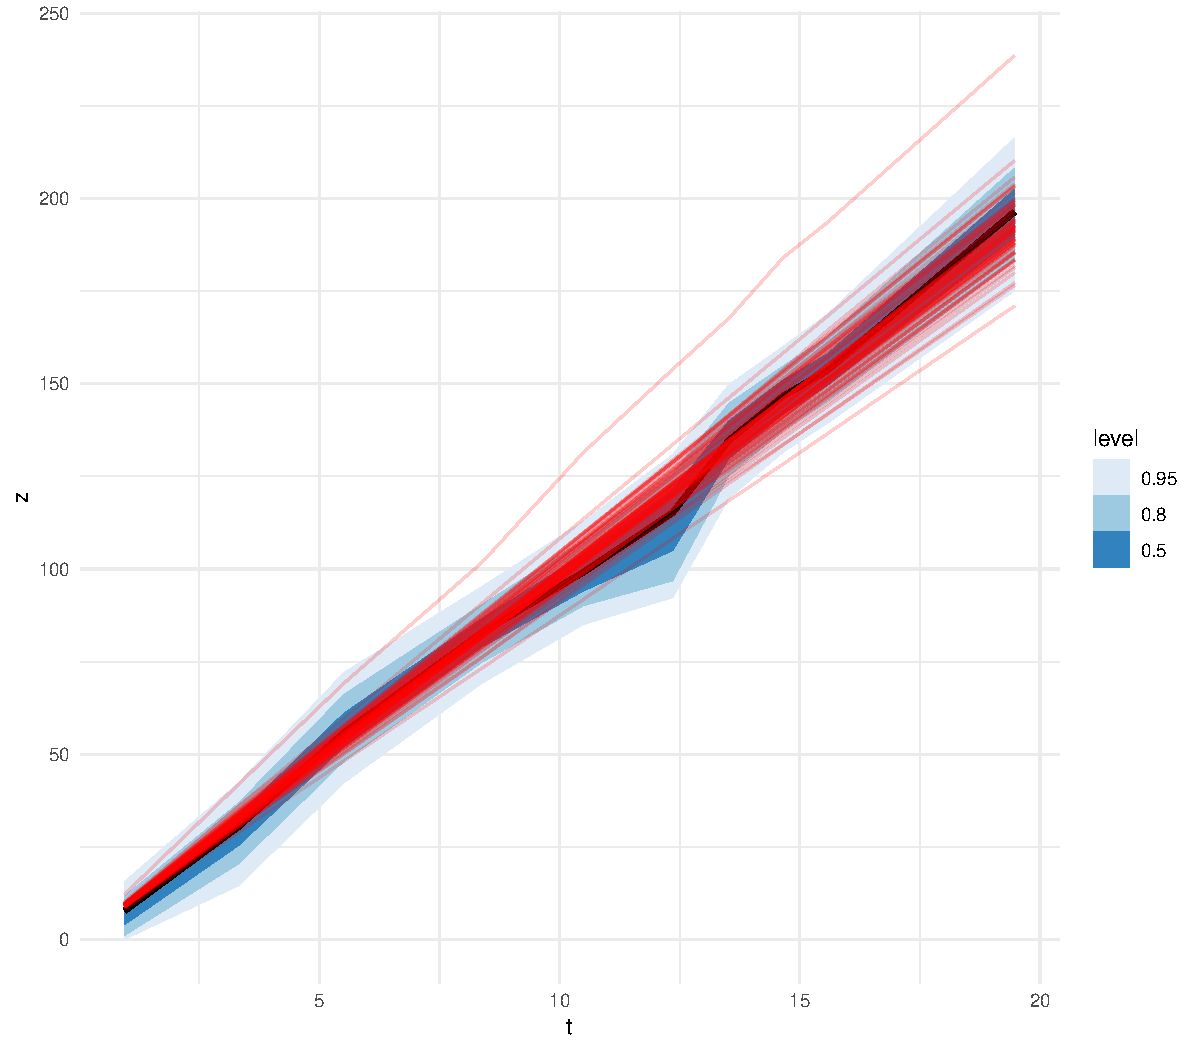
\includegraphics[width=0.8\columnwidth]{./figures/ch-4/zppd-divergencies.pdf}
  \caption{The divergent traces overlaid (in red) on the posterior predictive distribution of the degradation path for the small data set.}
  \label{fig:z-ppd-divergent}
\end{figure}

\paragraph*{Comparison of the two posteriors}
In comparison, this degenerate behaviour in the posterior is almost completely washed out by extra information in the large dataset. Figure~\ref{fig:z-jump-comparison} shows the joint distributions of the intermediate quantities $\Delta z_{15}$ ((a) and (c) in Fig.~\ref{fig:z-jump-comparison}) from the model conditioned on the big dataset and $\Delta z_{9}$ ((b) and (d) in Fig.~\ref{fig:z-jump-comparison}) for the small with $\log(\nu)$ and $\sigma$. In the two datasets, $\Delta z_{15}$ and $\Delta z_{9}$ are the same jump in degradation. In the joint posterior of $\Delta z_{9}$ and $\log(\nu)$ (Fig.~\ref{fig:z-jump-comparison}~(b)), there is the deep funnel shape around $\Delta z_{9} = 9$ and $\log(\nu) = -\infty$, and there is a second mode in the joint distribution of $\Delta z_{9}$ and $\sigma$ (Fig.~\ref{fig:z-jump-comparison}~(d)). However, in the joint distribution of $\Delta z_{15}$ and $\log(\nu)$ (Fig.~\ref{fig:z-jump-comparison}~(a)) there is very little mass around $\Delta z_{15} = 9$ and no second mode in the joint distribution of $\Delta z_{15}$ and $\sigma$ (Fig.~\ref{fig:z-jump-comparison}~(c)). This behaviour suggests the nonidentifiability only exists when there are few observations.

\begin{figure}
  \centering
  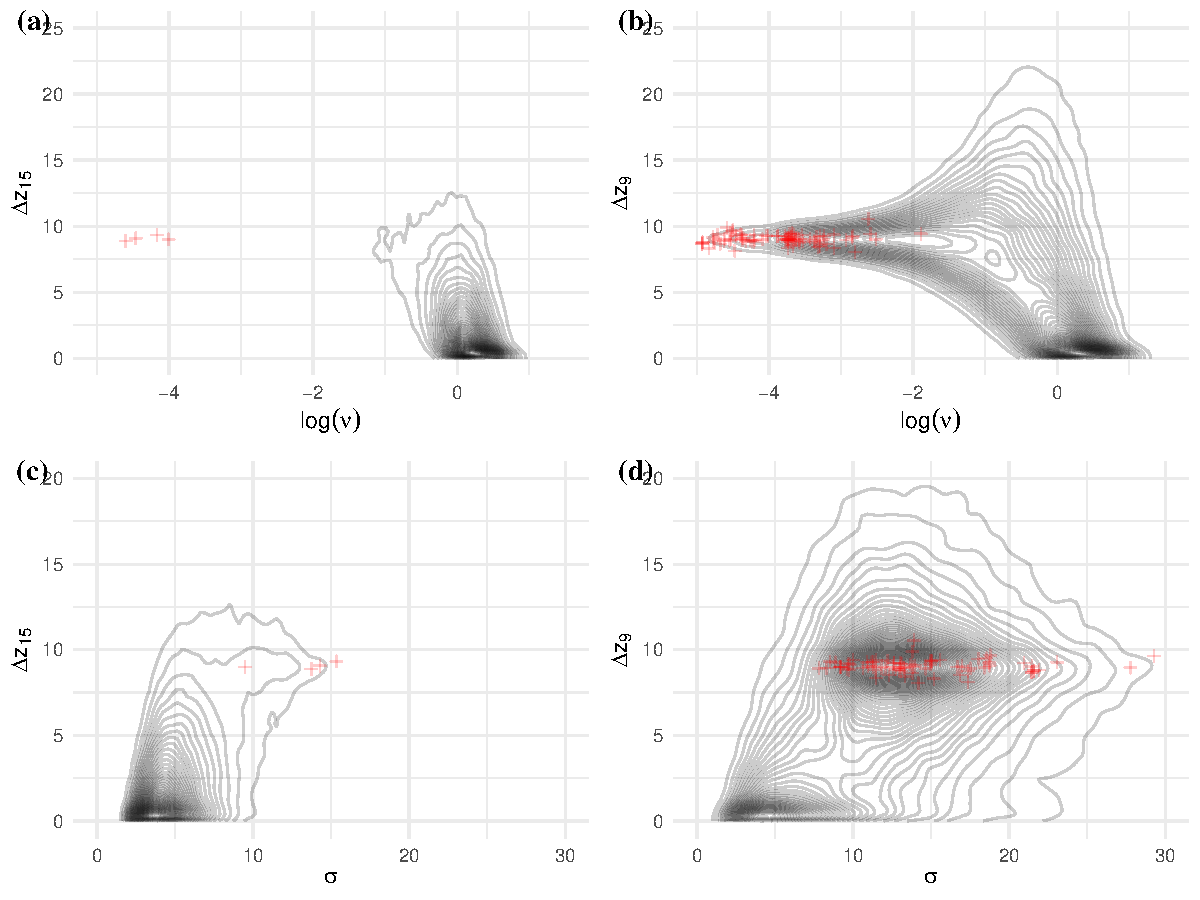
\includegraphics[width=0.95\columnwidth]{./figures/ch-4/joint-sig-jump.pdf}
  \caption{The contours of the posterior joint distribution of $\Delta z_{15}$ and $\log(\nu)$ (a) and $\Delta z_{15}$ and $\sigma$ (c) from the posterior when fit to all twenty observations and $\Delta z_{9}$ and $\log(\nu)$ (a) and $\Delta z_{9}$ and $\sigma$ (c) from the posterior when fit to only ten observations. The divergent transitions are overlaid in red and show the areas in the posterior that are dificult to sample from.}
  \label{fig:z-jump-comparison}
\end{figure}

\subsection{Solutions to computational issues} \label{sec:comp-sols}

The identifiability issues of the small data set can also be solved by injecting more information into the analysis that helps disentangle $\sigma$ and $\nu$. This information can come in the form of either supplementary data or prior information that informs one of the nonidentifiable parameters. Obtaining extra information about the measurement error would typically be much easier than the coefficient of variation of the gamma process. Here, I show that adding a small amount of supplementary information using either supplementary data or a stronger prior helps to identify $\sigma$ and, therefore, $\nu$, resulting in much smoother geometries in the posterior and, therefore, much more efficient sampling. The results regarding inference are arguably better than when I fit the model to all twenty degradation observations without supplementary information about $\sigma$.

\paragraph*{Prior information}

In Sec.~\ref{sec:noisy-GP-results}, I have used an effectively non-informative prior for the standard deviation of the measurement error. Typically, a technician would have some understanding of the variability in the measurement process. To emulate this, I place a Gaussian prior on the standard deviation of the measurement error
\begin{equation*}
  \sigma \sim \mbox{N}(4, 1).
\end{equation*}
This prior is centred around the true value of $\sigma$ and places $95\%$ of the mass between $\sigma = 2$ and $\sigma = 6$. Sampling from the posterior of the noisy gamma process model with a stronger prior, conditioning on the small dataset, is much quicker, and no divergent transitions occur. Figure~\ref{fig:energies-strong-prior} shows the chain energies of the sampler when a stronger prior is used on sigma. The marginal energy distribution and the first differenced distribution now match closely, showing that the chains have efficiently explored the posterior.

\begin{figure}
  \centering
  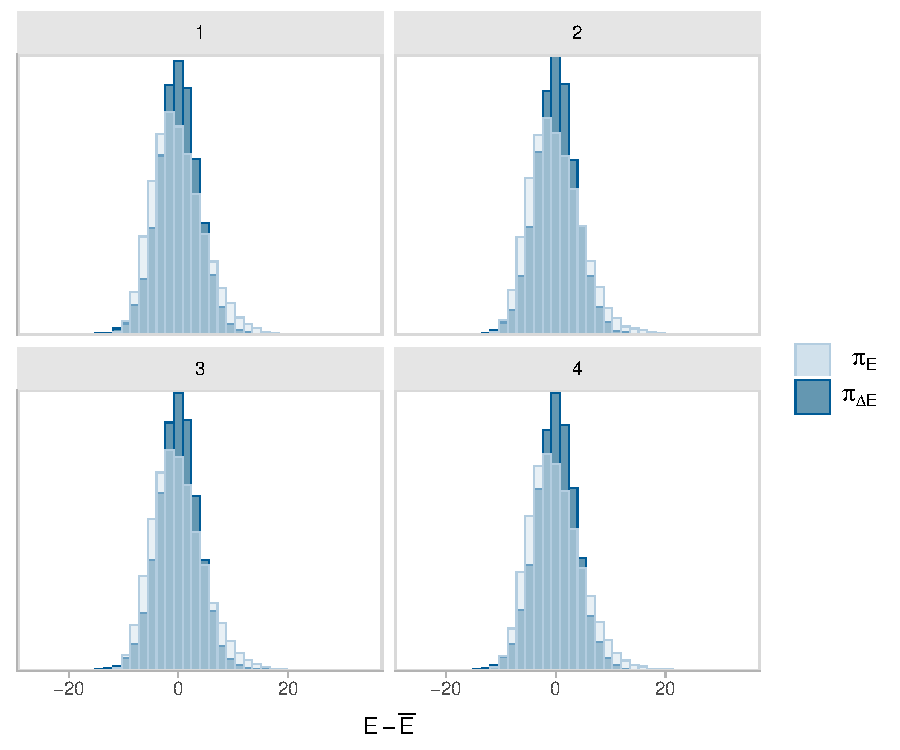
\includegraphics[width=0.8\columnwidth]{./figures/ch-4/strong-prior-nuts-energy.pdf}
  \caption{The chain energy diagnostics when the model is fit with a stronger prior on $\sigma$.}
  \label{fig:energies-strong-prior}
\end{figure}

A pairs plot of the MCMC samples is shown in Fig.~\ref{fig:pairs-strong-prior}. In the plots, the geometry looks much smoother than in Fig.~\ref{fig:pairs}, and there is little remanence of the deep funnel-shaped degeneracies between $\log{\nu}$ and $\mu$ and $\Delta z_1$. In Fig.~\ref{fig:marginal-post-extra-info}, I compare the marginal distribution for $\sigma$, $\mu$, and $\nu$ from this posterior with the true values and the model fits of Sec.~\ref{sec:noisy-GP-results}. The marginal distributions of the model with the stronger prior are much smoother, and there is now no mass around zero in the posterior of $\nu$.

\begin{figure}
  \centering
  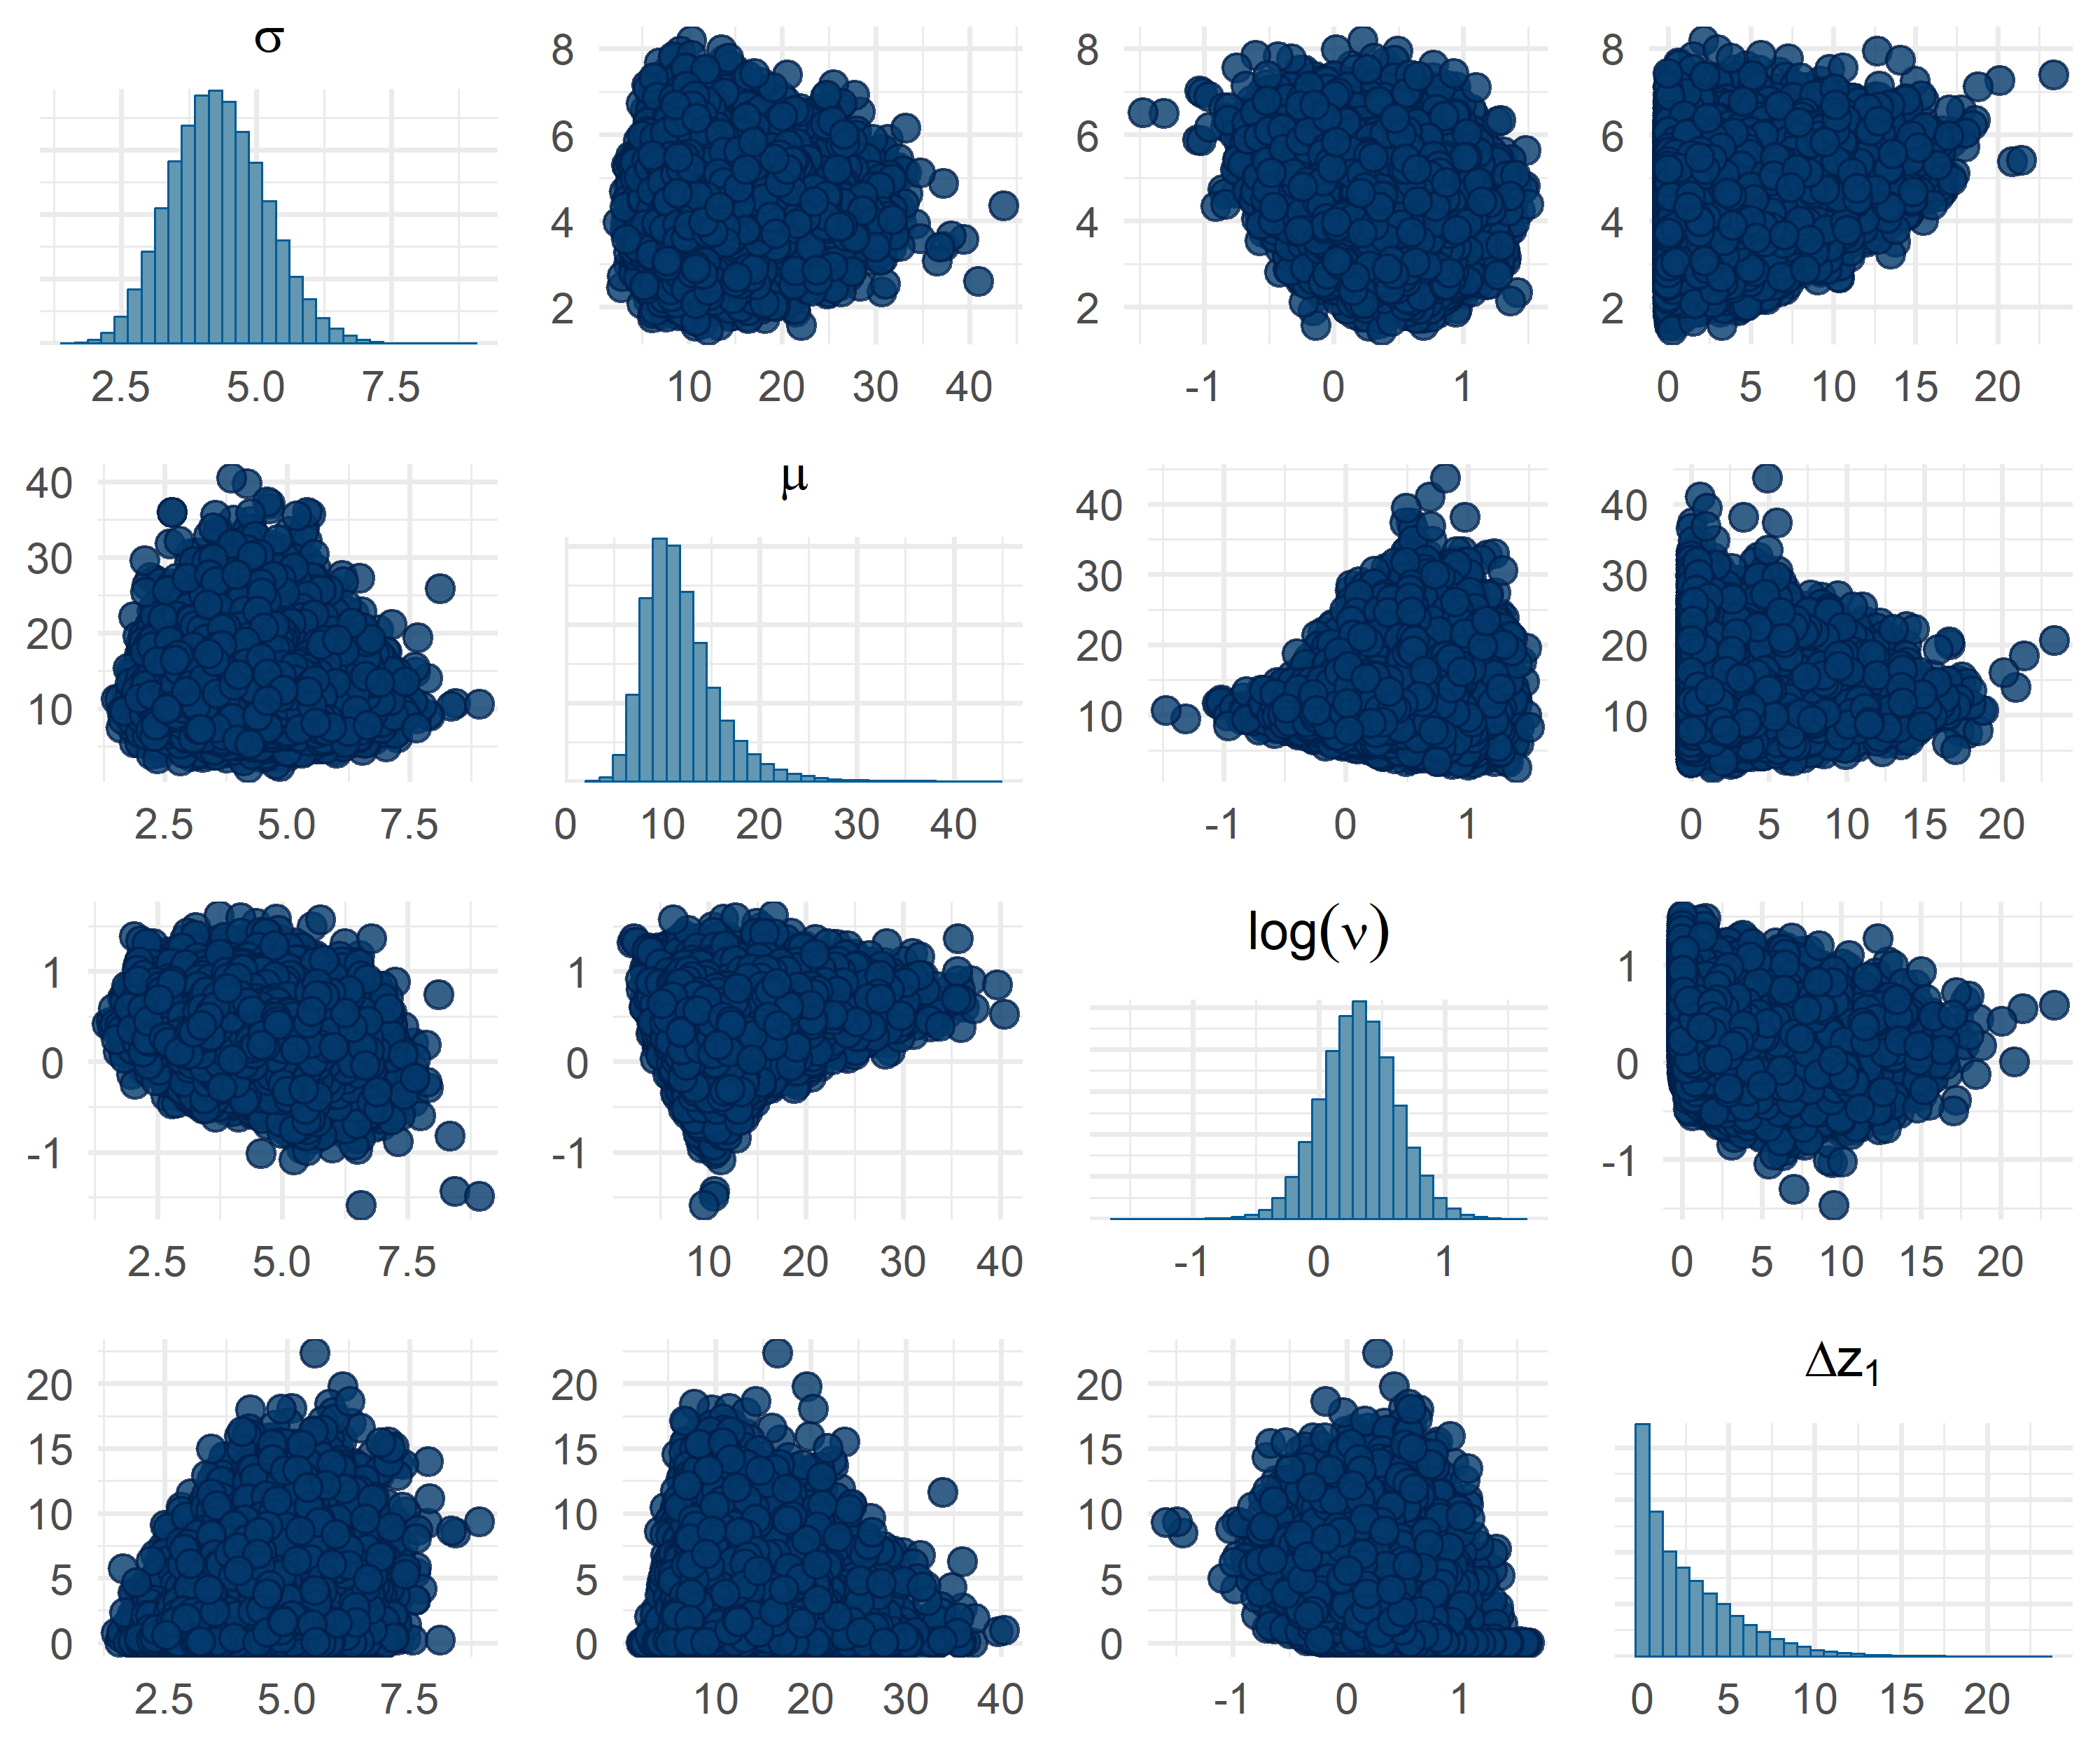
\includegraphics[width=0.8\columnwidth]{./figures/ch-4/strong-prior-pairs.png}
  \caption{The pairs plot of the MCMC draws when using a stronger prior on $\sigma$.}
  \label{fig:pairs-strong-prior}
\end{figure}

\paragraph*{Supplementary data}

As an alternative to using a stronger prior, extra data that informs $\sigma$ can be used to improve the behaviour of sampling. I sample five supplementary observations of the measurement error from the distribution
\begin{equation*}
 y_{\text{\tiny{sup}}} \sim \mbox{N}(0, 4).
\end{equation*}
Extra supplementary observations such as these could be obtained by taking multiple measurements at time $t = 0$, when the degradation is known to be zero, just before decommissioning the component---after which detailed non-noisy measurements can be obtained---or by performing a small experiment. The supplementary observations can be easily incorporated into the Hierarchical model by extending the data model to
\begin{align*}
 y_i|z_i, \sigma & \sim \mbox{N}(z_i, \sigma) && \mbox{data model} \\
 y_{\text{\tiny{sup}}} & \sim \mbox{N}(0, \sigma).
\end{align*}
Similar to the more informative prior, the sampler is much more efficient, no divergencies occur during sampling, and the geometry of the posterior distribution looks much smoother (not shown). The resulting marginal posterior distributions of $\sigma$, $\mu$, and $\nu$ for the model fit with both the small dataset and the supplementary data are also compared in Fig.~\ref{fig:marginal-post-extra-info}. The marginal distributions of the parameters are very much the same as when a stronger prior is used, and the model successfully reclaims the true parameter values.

\begin{figure}
  \centering
  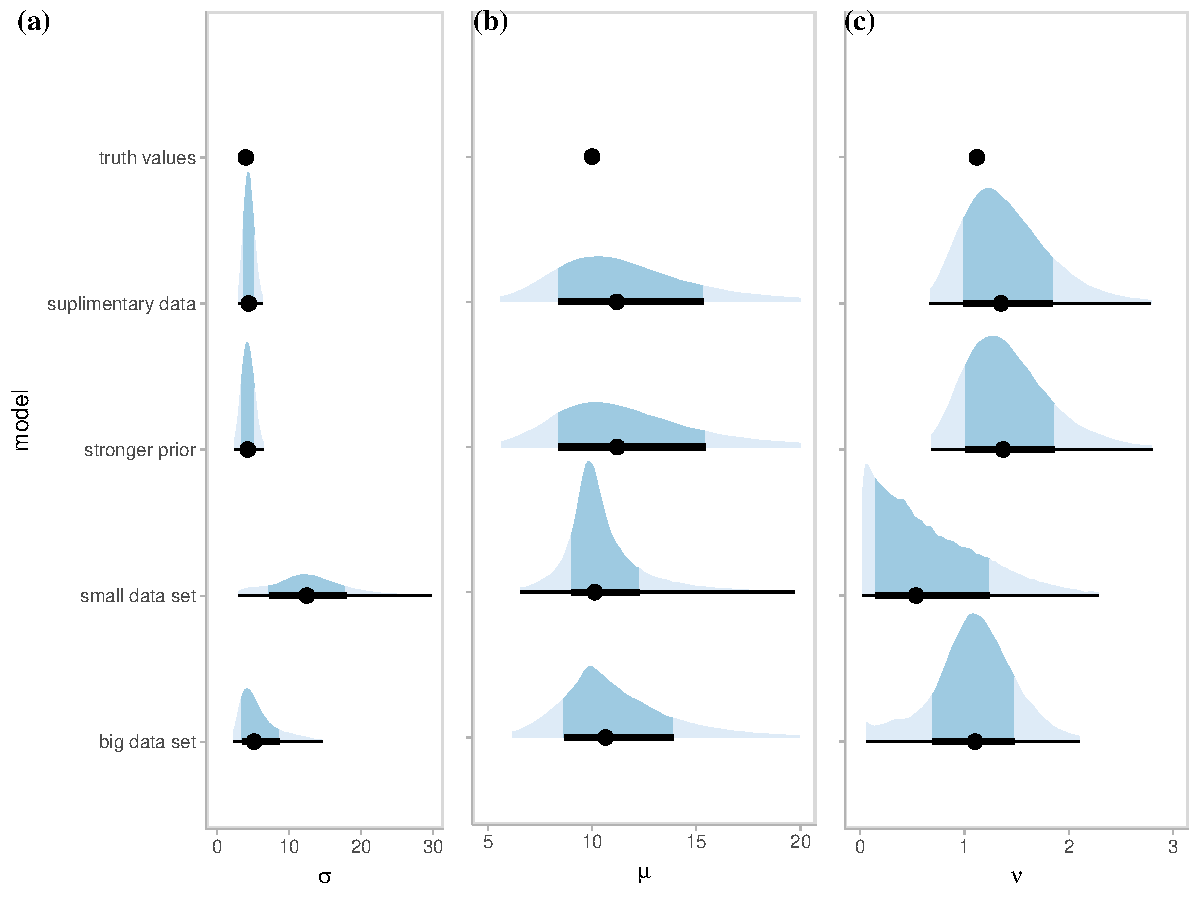
\includegraphics[width=0.8\columnwidth]{./figures/ch-4/marginal-post-extra-info.pdf}
  \caption{The marginal posterior distributions of the parameters $\sigma$, $\mu$, and $\nu$ when information is added into the analysis either through a stronger prior or supplementary data compared to the original two posteriors.}
  \label{fig:marginal-post-extra-info}
\end{figure}

\section{Discussion} \label{sec:NGP-discussion}

The main focus of this chapter was to show that using the Bayesian hierarchical formalism allows us to frame a model for a noisy gamma stochastic process in a tractable and transparent manner. Decomposing the noisy gamma process into a sequence of conditional models---the data, process, and parameter models---removes the need for complex deconvolutions that require the evaluation of, or approximations to, multidimensional integrals. Making this connection that allows the simple extension of the GP to noisy degradation observation and showing its implementation in the contemporary Bayesian computational environment Stan, is a step towards making stochastic degradation models applicable to use in industry and also accessible to practitioners. Below, I summarise the main element of this chapter and highlight the important findings and contributions, as well as areas for future work.

Reparameterising the gamma process in terms of the mean $\mu$ and coefficient of variation $\nu$ results in more interpretable parameters than the shape $\beta$ and rate $\xi$: $\mu$ is the mean wear rate, and $\nu$ is the inverse of the `signal-to-noise' ratio, and hence is a measure of the volatility of the gamma process. The interpretability of $\mu$ and $\nu$ simplifies specifying prior distributions because they are easier to elicit domain information about. Additionally, reparameterising the gamma process in this way also helps clarify how extensions of the model, such as unit-to-unit variability (which I show in the next chapter) or covariates, can be incorporated into the model. Finally, the parameters $\mu$ and $\nu$ are orthogonal, which has desirable computational benefits.

Under this new parameterisation, I re-assessed good choice of priors and showned a principled way of assessing these priors. I draw away from the conventional gamma priors used for the gamma process and think deeply about the justification of priors to construct a weakly informative set of prior distributions that conform with my understanding of the underlying data-generating process. I then evaluate if the priors are, in fact, weakly informative through prior predictive checking. The use of a weakly informative prior is particularly important in the case of a noisy gamma process, since the noisy observation of the degradation trace means that the data do not strongly inform the underlying degradation model and in such cases using non-informative prior distributions can put large amounts of mass in unrealistic parts of parameter space \citep{tian2024}.

In fitting the proposed noisy gamma process to simulated data, I identify issues with sampling from the posterior when there are only a few observations. Investigating the poor sampling uncovers an identifiability issue between the volatility of the gamma process (expressed by $\nu$) and the measurement error ($\sigma$), which is only present when the sample size is small. The observed degenerate behaviour of inference from the small-data posterior results from what \citet{betancourt_2020} refers to as `pre-asymptotic non-identifiability'.

Because variation in the noisy degradation signal can be a result of both the randomness of jumps of the GP and the randomness of the measurement error, it can be difficult to separate these two sources when there is only a small number of observations. In the small dataset, the data do not strongly inform the parameters $\sigma$ and $\nu$, and it is therefore difficult to distinguish between competing models---the noisy gamma process and one where $\nu$ approaches zero---as reflected in their multi-modal posterior distributions. Using the terminology of \citet{betancourt_2020}, we can say that these parameters are pre-asymptotically non-identifiable.

I further confirm this in Sec.~\ref{sec:comp-sols} by showing that the computational issues and pathological behaviour in the posterior are completely resolved by adding additional information that specifically informs one of the pre-asymptotically non-identifiable parameters. Although fitting the model to all twenty noisy observations results in a much better behaved posterior than fitting it to only ten, there are still remanence of the degenerate areas seen in the posterior conditioned on only ten observations; in addition, there are still a few divergencies and the chain energy plots (Fig.~\ref{fig:nuts-energies}) show that sampling is still slow. In contrast, when I use a stronger prior for $\sigma$ or add a small amount of supplementary data that informs $\sigma$, there is no sign of degenerate behaviour in the posteriors and sampling becomes very efficient. With enough noisy observations, the model eventually becomes identifiable from the noisy degradation data alone. However, in a typical reliability application, the analysis will have small sample sizes, in which case adding additional information to the analysis can help to identify the model.

The issue of pre-asymptotically non-identifiability is not unique to the noisy gamma process. In an early paper on noisy Wiener processes, \citet{whitmore_1995} also remarked on the difficulty in estimating the measurement error variance of a noisy Wiener process. In a Bayesian reanalysis of the same data, \citet{hamada_2008} imposed strong prior distributions on the measurement error variance and the variance of the Wiener process in order to ensure identifiability, although they do not explicitly justify their reasons for doing so. More work should be done to understand the interplay between the scale of the measurement error, the volatility of the underlying stochastic degradation process, and these small sample identifiability issues.

In the context of real noisy degradation data, there is no way of checking if there is enough information in the data to properly identify the model. Therefore, practitioners applying the noisy GP model should use as much information as they have available to them. This includes encoding their domain-expert knowledge into the prior distributions of the parameters, rather than choosing a default non-informative prior; incorporating supplementary data that informs one of the pre-asymptotically non-identifiable parameters; and, if available, modelling the degradation of groups of similar units jointly as to `borrow' information. With respect to the latter, in the next chapter, I extend the noisy gamma process for a single degradation trace to model noisy degradation paths from multiple units while assuming that the measurement error is the same for all units. Doing so pools information from between multiple units to inform the parameters, drastically improving the problems with identifiability and MCMC sampling that I have demonstrated in this chapter.